\documentclass[12pt,titlepage,twoside]{article}
\usepackage{titlesec}
\usepackage{blindtext}

\usepackage{german}				% deutsche Überschriften etc.
\usepackage[utf8]{inputenc}		% direkte Einbgabe von Umlauten

% Layout-Einstellungen
\frenchspacing					% no extra space after periods
\usepackage{parskip}			% paragraph gaps instead of indentation
\usepackage{mathptmx}			% supposed to replace \usepackage{times}
\usepackage[scaled=0.9]{helvet}	% supposed to replace \usepackage{times}
\usepackage{courier}			% supposed to replace \usepackage{times}
\tolerance=9000					% avoid words across right border

% miscellaneous
\usepackage{graphicx}			% save svg with dia -> use inkscape to save as pdf
\usepackage{svg}
\usepackage{rotating}
\usepackage{wrapfig}
\usepackage{hhline}				% double lines in tables
\usepackage{amsfonts}			% real numbers etc.
\usepackage[rightcaption]{sidecap}	% figure captions on the right (optional)
\usepackage{listings}			% for code samples
\lstset{
    escapeinside={(*@}{@*)}
}
\renewcommand{\lstlistlistingname}{Listingverzeichnis}	% header name for the list of listings

\usepackage{spverbatim}

\usepackage{fancyhdr}			% for header line
\usepackage{booktabs}
\usepackage{float}


\usepackage{diagbox}			% diagonal table cell lines

\usepackage{geometry}

\geometry{a4paper,left=25mm, right=25mm, top=3.0cm, bottom=2.5cm}
\usepackage{tabularx}
% Kopf- und Fußzeile
\fancyhead{} % clear all header fields
\fancyhead[OR,LE]{\leftmark}

\usepackage{hyperref}			% for clickable references
\hypersetup{
	linktoc=all,
	colorlinks,
	citecolor=black,
	filecolor=black,
	linkcolor=black,
	urlcolor=black,
	plainpages=false
}

\usepackage{cite}
\renewcommand{\UrlBreaks}{\do\/\do\-\do\_}	% allows URL breaking on /, - and _
\usepackage{breakurl}

\usepackage[toc,page]{appendix}
\usepackage[nottoc]{tocbibind}

\usepackage{etoolbox}	% may already be loaded by bibtex
\patchcmd{\thebibliography}{\clubpenalty4000}{\clubpenalty10000}{}{}	% avoid breaking bib entrys
\patchcmd{\thebibliography}{\widowpenalty4000}{\clubpenalty10000}{}{}	% avoid breaking bib entrys

\newlength\tdima
\newcommand\tabfill[1]{
      \setlength\tdima{\linewidth}
      \addtolength\tdima{\@totalleftmargin}
      \addtolength\tdima{-\dimen\@curtab}
      \parbox[t]{\tdima}{#1\ifhmode\strut\fi}}

\newcommand*{\reflabel}[1]{\hyperref[{#1}]{\ref*{#1} \nameref*{#1}}}
\newcommand*{\reftype}[1]{\hyperref[{#1}]{\autoref*{#1}}}
\newcommand*{\refcomplete}[1]{\hyperref[{#1}]{\autoref*{#1} \nameref*{#1}}}

\renewcommand{\contentsname}{Inhaltsverzeichnis}
\renewcommand\appendixtocname{Anhang}
\renewcommand\appendixpagename{Anhang}

\def\postbreak{
  \raisebox{0ex}[2.0ex][0.5ex]{\ensuremath{\color{red}\hookrightarrow\space}}}

\lstdefinelanguage{JavaScript}{
  keywords={typeof, new, true, false, catch, function, return, null, catch, switch, var, if, in, while, do, else, case, break},
  keywordstyle=\color{blue}\bfseries,
  ndkeywords={class, export, boolean, throw, implements, import, this},
  ndkeywordstyle=\color{darkgray}\bfseries,
  identifierstyle=\color{black},
  sensitive=false,
  comment=[l]{//},
  morecomment=[s]{/*}{*/},
  commentstyle=\color{purple}\ttfamily,
  stringstyle=\color{red}\ttfamily,
  morestring=[b]',
  morestring=[b]"
}

\title{Design und Implementierung einer Serverless-Architektur am Beispiel des Cloud Providers Amazon Web Services}
\newcommand{\titleEnglish}{Design and implementation of a serverless architecture using the example of the cloud provider Amazon Web Services}

\author{Oktavius Wiesner}
\newcommand{\Matrikelnummer}{1082104}
\date{\today{}, Duisburg}

\makeatletter
%%%%%%%%%%%%%%%%%%%%%%%%%%%%%%%%%%%%%%%%%%%%%%%%%%%%%%%%%%%%
\begin{document}

\bibliographystyle{amsalpha}
\definecolor{flashwhite}{rgb}{0.95, 0.95, 0.96}
\definecolor{dkgreen}{rgb}{0,0.6,0}
\definecolor{gray}{rgb}{0.5,0.5,0.5}
\definecolor{mauve}{rgb}{0.58,0,0.82}
\definecolor{lightgray}{rgb}{.9,.9,.9}
\definecolor{darkgray}{rgb}{.4,.4,.4}
\definecolor{purple}{rgb}{0.65, 0.12, 0.82}
\definecolor{ashgrey}{rgb}{0.7, 0.75, 0.71}
\definecolor{lavender}{rgb}{0.9, 0.9, 0.98}

\pagenumbering{roman}	% Start roman numbering - 'Roman' for uppercase


%-------------------------------------------------------------

\begin{titlepage}

\begin{center}
{\Large\bf \@title}\\[3cm]



{\bf Bachelorarbeit}\\
zur Erlangung des Grades {\em Bachelor of Science}\\[1.5cm]

an der\\
Hochschule Niederrhein\\
Fachbereich Elektrotechnik und Informatik\\
Studiengang {\em Informatik}\\[3cm]

vorgelegt von\\
\@author\\
Matrikelnummer: \Matrikelnummer\\[3cm]
Datum: \today\\[3cm]

Prüfer:~Prof.~Dr.~Peter Davids
\\Zweitprüfer:~Maik Glatki

\end{center}
\end{titlepage}

\pagestyle{empty}
\clearpage

%-------------------------------------------------------------


%-------------------------------------------------------------

%-------------------------------------------------------------
\section*{Abstract}
%-------------------------------------------------------------

Die vorliegende Bachelorarbeit beschäftigt sich im Detail mit dem Thema Serverless und dem zugehörigen Modell Function as a Service.
Zur Verständlichkeit werden die verschiedenen Servicemodelle des Cloud Computings vorgestestellt und verglichen.

Die Bachelorarbeit beschränkt sich auf den Cloud Provider Amazon Web Services und der entsprechenden Dienste, die für den Einsatz von Serverless Anwendungen zur Verfügung stehen.
Dabei werden AWS-Dienste wie Lambda, Cognito, AppSync, DynamoDB und Amplify genauer untersucht und bewertet.
Auf Basis der untersuchten Dienste wird ein Prototyp bei AWS entwickelt und implementiert. Die Programmiersprache ist bei der Implementierung NodeJS bzw. Javascript und React.
Das Ziel ist eine moderne Web Applikation für die Mitarbeiter der Mediengruppe RTL, die komplett auf Serverless Architektur basiert
und die in der Bachelorarbeit erwähnten Vorteile vollständig ausnutzen kann.




\clearpage

%-------------------------------------------------------------


%-------------------------------------------------------------

%-------------------------------------------------------------
\section*{Eidesstattliche Erklärung}
%-------------------------------------------------------------
%\begin{tabbing}
%Name: \hspace{4em}\= \@author\\
%Matrikelnr.: \> \Matrikelnummer\\
%Titel: \> \@title
%\end{tabbing}

\begin{table}[h]
\begin{tabularx}{\textwidth}{l X}
Name:			& \@author \\
Matrikelnr.:	& \Matrikelnummer \\
Titel:			& \@title 

				\titleEnglish \\
\end{tabularx}
\end{table}

Ich versichere durch meine Unterschrift, dass die vorliegende Arbeit
ausschließlich von mir verfasst wurde.
Es wurden keine anderen als die von mir angegebenen Quellen und Hilfsmittel
benutzt.

Die Arbeit besteht aus \underline{\hspace{3em}} Seiten.

\vspace{8ex}
\begin{tabbing}
\underline{\hspace{14em}} \hspace{3em}\= \underline{\hspace{14em}} \\
Ort, Datum \> Unterschrift
\end{tabbing}





\cleardoublepage





%-------------------------------------------------------------


%-------------------------------------------------------------
\section*{Hinweis}

Bei allen Ausführungen im Folgenden, die auf Personen bezogen sind, meint die
gewählte Formulierung beide Geschlechter, auch wenn aus Gründen der
sprachlichen Vereinfachung und der besseren Lesbarkeit die männliche Form
gewählt wurde.

\clearpage
%-------------------------------------------------------------


%-------------------------------------------------------------
%-----\section*{Danksagung}

Hier kommt eine Danksagung...






%-----\clearpage
%-------------------------------------------------------------

\pagestyle{fancy}
\tableofcontents

\clearpage
\pagestyle{empty}

\clearpage


%-------------------------------------------------------------
% default a), b), c) numbering
\renewcommand{\labelenumi}{\alph{enumi})}
\pagenumbering{arabic} % Switch to regular numbers
%=============================================================


%%%%%%%%%%%%%%%%%%%%%%%%%%%%%%%%%%%%%%%%%%%%%%%%%%%%%%%%%%%%%%%%%%%%%%%%%%%%%%%%
\pagestyle{fancy}
\fancyhf{}

\fancyhead[OR]{Einleitung}
\fancyhead[ER]{Einleitung}
\fancyfoot[C]{\thepage}


\section{Einleitung}

\subsection{Aufgabenstellung}

Das Ziel dieser Bachelorarbeit ist es die Serverless Architektur zu bewerten und einen Prototyp für die Abteilung Datacenter and Clouds der Firma CBC Cologne Broadcasting GmbH (Im folgenden \glqq CBC\grqq) zu erstellen.
Der Fokus soll hierbei gleichmäßig auf das Design der Anwendung als auch auf der Implementierung gelegt werden.

Im ersten Schritt soll überprüft werden, inwieweit sich die gewünschte Anwendung mit Serverless Diensten realisieren lässt.
Anschließend sollen alle potenziellen Dienste des Cloud Providers Amazon Web Services (Im folgenden \glqq AWS\grqq) untersucht werden und die geeignetsten ausgewählt werden.

Bei der Implementierung sollen diese Dienste dann in der Praxis angewandt werden. Für das Frontend soll ein modernes Framework verwendet werden.
Die Implementierung soll möglichst allgemein verwirklicht werden, sodass jeder Mitarbeiter der Abteilung Datacenter and Clouds in Zukunft an dieser Anwendung weiter arbeiten kann.



\subsection{Motivation}
\label{Motivation}
Die Abteilung Datacenter and Clouds innerhalb von CBC beschäftigt sich mittlerweile seit einigen Jahren mit Cloud Infrastruktur.
Zu Beginn wurden größenteils dynamisch Linux Server mit einer Datenbank und einem Loadbalancer realisiert(Infrastructure as a Service).
Mit der Zeit wurden auch Container-basierte Varianten mit Docker sowie Platform as a Service Lösungen umgesetzt.
Function as a Service wurde bisher nur mit Amazon Web Services Dienst Lambda realisiert.
Mittlerweile gibt es den Wunsch sich intensiv mit Function as a Service zu beschäftigen um vor allem eine schnelle Bereitstellung von Diensten zu geringen Kosten zu ermöglichen.
Webanwendungen sollen schneller bereitgestellt werden, ohne dass Server konfiguriert und gewartet werden müssen.

Da sehr viele Firmen innerhalb der Mediengruppe RTL intensiv mit AWS und anderen Cloud Providern arbeiten ist die Kostenzuweisung unübersichtlich geworden.
Jeder Cloud Provider stellt seine Abrechnungen auf unterschiedliche Weise dar und alle Daten müssen unterschiedlich aufbereitet werden.
AWS exportiert die Abrechnungen monatlich in dem Cloud-Speicher
S3\footnote{S3 steht für Simple Storage Service und ist ein Objektspeicherservice von Amazon, für eine beliebe Menge von Daten.
Daten werden in S3 Buckets abgelegt und können aus dem Internet abgerufen werden.
CBC verwendet S3 für viele unterschiedliche Szenarien, darunter auch das Speichern von Videodateien für den Dienst TVNow.   }, wohingegen Google Cloud Plattform alle Daten in ein SQL ähnliches Data Warehouse speichert.
Zudem ist es notwendig innerhalb der Mediengruppe RTL intern Abteilungen zuzuweisen und abzuschreiben.

Deshalb besteht innerhalb der Abteilung Datacenter and Clouds der Wunsch nach einer modernen Web Applikation, welche die Informationen der jeweiligen Cloud Provider zentral sammelt und zur Verfügung stellt.
Zu den Informationen gehören Daten zu den Kosten, Abrechnungen, verwendete Ressourcen und nach Bedarf weitere.
Im Rahmen der Bachelorarbeit soll dafür ein Prototyp entstehen der effizient und einfach in Zukunft um weitere Anforderungen erweitert werden kann.


\subsection{CBC Cologne Broadcasting GmbH}

Die Bachelorarbeit wird innerhalb der Räumlichkeiten des Unternehmens CBC Cologne Broadcasting GmbH in Köln Deutz realisiert.
CBC ist ein Unternehmen der Mediengruppe RTL Deutschland, welches wiederum zur Bertelsmann-Tochter RTL Group in Luxemburg gehört.
Neben CBC gehören unter anderem der Werbezeitenvermarkter IP Deutschland sowie die Fernsehsender RTL Television, RTL Nitro, N-TV und Vox zur Mediengruppe RTL.


Mit ca. 550 festen Mitarbeitern ist CBC für die Produktion, Programmverbreitung, Sendeabwicklung sowie die IT Infrastruktur verantwortlich.
Neben der Betreuung von Projekten innerhalb der Mediengruppe RTL ist die CBC auch für die Berichterstattung der Fußball-Bundesliga verantwortlich.
Die Abteilung Datacenter and Clouds beschäftigt sich dabei mit Infrastrukturthemen, sowohl On Premises als auch bei den Cloud Providern Amazon Web Services, Microsoft Azure sowie Google Cloud Platform.
Beispiele für Projekte, die in der Cloud umgesetzt wurden sind die Streaming-Plattform TVNOW sowie die Internetpräsenz des Nachrichtensenders N-TV.
Gegründet wurde die CBC 1994 in Köln, Geschäftsführer ist Thomas Harscheidt.


\subsection{Gliederung}

Diese Bachelorarbeit gliedert sich in fünf Kapitel.

Im ersten Kapitel wird mit einer Einleitung sowie grundlegenden Informationen zum Inhalt der Bachelorarbeit und den allgemeinen Rahmenbedingungen ein Ausblick auf den weiteren Verlauf gegeben.

Anschließend werden alle grundlegenden Begriffe und Cloud Modelle erläutert und miteinander verglichen, bevor genauer auf das Thema Serverless eingegangen wird.
Hier wird auch die Eignung der Architektur thematisiert.

Nach diesem Abschnitt wird im Detail auf die verschiedenen Serverless-Dienste beim Cloud Provider Amazon Web Services eingegangen und begründet, warum die ausgewählten Dienste für diese Bachelorarbeit am besten geeignet sind.
Zusätzlich wird die Auswahl der Programmiersprache sowie des Frameworks besprochen.

Das darauf folgende vierte Kapitel beschreibt die Implementierung der gewählten Dienste im Detail. Dazu wird der geschriebene Code vorgestellt und der Verlauf aufgezeigt.

Abschließend dient das fünfte Kapitel der Diskussion und gibt einen Ausblick in die Zukunft des Systems.
Hier befindet sich ebenfalls eine Zusammenfassung inklusive einem Fazit der Bachelorarbeit.
Außerdem werden die bisher angefallenen Kosten des Prototyps dargestellt.



\clearpage

\fancyhead[OR]{Cloud Computing und Serverless}
\fancyhead[ER]{Cloud Computing und Serverless}
\fancyfoot[C]{\thepage}
\section{Cloud Computing und Serverless}

\subsection{Allgemeines}

Bevor man sich mit dem Design und der Implementierung von Serverless Architektur beschäftigen kann, ist es notwendig sowohl Begriffe wie Cloud Computing und Serverless zu erklären als auch alle wichtigen Cloud Computing-Modelle darzustellen und miteinander zu vergleichen.

Das Modell Function as a Service ist eine logische Fortführung der bisher existierenden Servicemodelle.
Somit sind auch diese Grundvoraussetzung für das Thema Serverless
Im folgenden Abschnitt werden all diese erforderlichen Voraussetzungen geschaffen und die einzelnen Cloud Computing-Modelle miteinander verglichen.


\subsection{Definition und Erläuterung}
Der Begriff Cloud Computing beschreibt im Wesentlichen die Bereitstellung von Rechnerressourcen über das Internet.
Hierbei kann es sich um jede Art von Ressourcen handeln. Dazu zählt zum Beispiel die Netzwerkinfrastruktur, Server, Speicher, Datenbanken aber auch Software.
Anwender zahlen nur die tatsächlich genutzte Leistung und können den Bedarf jederzeit flexibel anpassen.
Lokal muss in der Regel nur ein geeigneter Client installiert sein, etwa ein Webbrowser.

Die wichtigsten Vorteile gegenüber einer On Premises-Landschaft sind die schnelle Verfügbarkeit und Skalierung von Diensten, sowie keine Kosten im Voraus.
Durch den Einsatz von Cloudtechnologien verlagert sich das Kostenmodel von Capex\footnote{ Capex(Capital Expenditure) bezeichnet Investitionen und Ausgaben die einmalig getätigt werden
um den Umsatz zu erhöhen. Dazu gehört zum Beispiel die Anschaffung von neuer Hardware. } zu Opex\footnote{Opex(Operational Expenditure) bezeichnet wiederkehrende Kosten wie Verwaltungs- und Betriebskosten.
Auch fallen mittlerweile viele Softwarelizenzen regelmäßig an. }.
Mit einem Knopfdruck ist es möglich beliebig\footnote{Das Wort beliebig ist nicht sinngemäß zu verstehen.
Auch Cloud Provider haben nur eine endliche Anzahl von Kapazitäten und geben den Kunden diese nicht in vollem Ausmaß frei.
Jede Umgebung eines Kunden hat bestimmte Limitierungen pro Service, die jedoch bei Bedarf eventuell angepasst werden können.
AWS erlaubt beispielsweise pro Region und Account 2880 vCPUs für Standardinstanzen } viele Ressourcen und Dienste hochzufahren und zu verwenden.
Je nach Servicemodell verschiebt sich der Verantwortlichkeitsbereich zwischen dem Cloud Provider und dem Anwender.
\cite[]{CloudComputingDef}

\clearpage

\subsection{Cloud Computing-Modelle}
Zur Veranschaulichung der unterschiedlichen Servicemodelle dient folgende Grafik.
Im Anschluss werden die einzelnen Modelle im Detail beschrieben.


\begin{figure}[htbp]
    \centering
    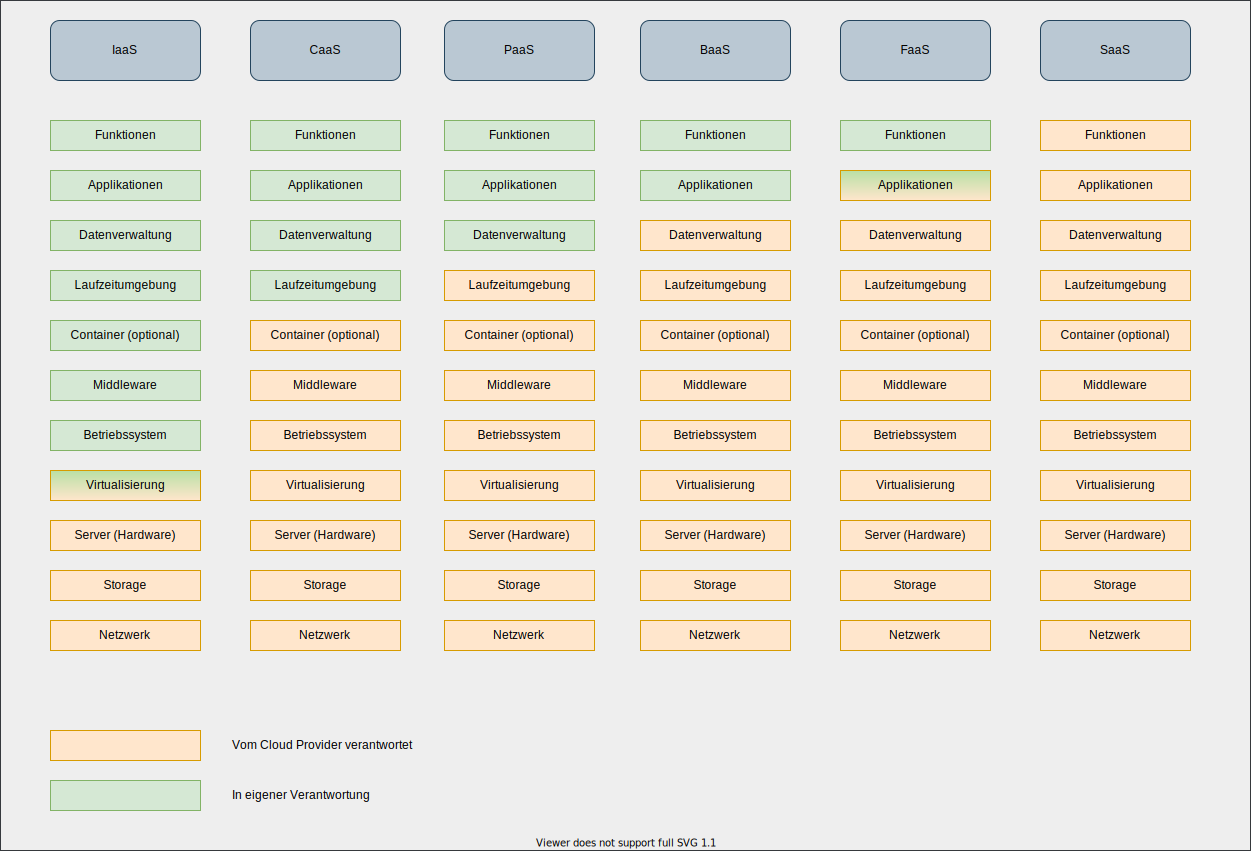
\includegraphics[width=1.0\textwidth]{30-Serverless-Theorie/ServiceModelle.png}
    \caption{Übersicht der Servicemodelle}
    \label{fig:meine-grafik}
\end{figure}


   \subsubsection{IaaS: Infrastructure as a Service}
   Unter dem Begriff Infrastructure as a Service, kurz IaaS, versteht man Infrastruktur bei der Administratoren bzw. Anwender sowohl die größte Kontrolle als auch die höchste Verantwortung tragen.
   Der Cloud Provider kümmert sich nur um die nötige Infrastruktur um Computing-Ressourcen über das Internet zur Verfügung stellen zu können.
   Dazu gehört der Erwerb und Betrieb von Servern, Switchen, Routern und Speichersystemen und der Virtualisierung von Maschinen.(siehe Abbildung 1).
   Dieses Modell ist am ehesten mit einer On Premises Infrastruktur vergleichbar.
   Der größter Vorteil jedoch sind die Initialkosten und das Investitionsrisiko.
   Ist man sich unsicher über die benötigte Rechenleistung oder schwankt diese häufig kann man jederzeit Ressourcen terminieren und Geld sparen.

   Das Betriebssystem inklusive aller damit verbunden Updates, die Regelung aller Zugriffe sowie die Installation und Wartung von Software liegen im Verantwortungsbereich des Kunden.
   Dieses Modell wird häufig verwendet wenn man eine Hybridlösung mit einer On Premises Landschaft aufbauen möchte oder die eigene Applikation noch nicht für die Anwendung in der Cloud optimiert wurde, man diese aber trotzdem in die Cloud migrieren möchte.\cite[]{CloudComputingDef}

   \subsubsection{CaaS: Container as a Service}
   Container as a Service bezeichnet das Bereitstellen sämtlicher Ressourcen zur Verwaltung von Containern und der dort installierten Software.
   Unter Container versteht man ein {}\glqq Standardsoftwarepaket \grqq{} welches {}\glqq den Code einer Anwendung zusammen mit den zugehörigen Konfigurationsdateien,
   Bibliotheken und den für die Ausführung der Anwendung erforderlichen Abhängigkeiten \grqq{} bündelt. \cite[]{CaaS}
   Dieser gebündelte Container ist leicht portierbar und die Ausführung erfolgt in einer konsistenten Umgebung.

   Der bekannteste Dienst Docker unterstützt Windows und Linuxsysteme, sowohl OnPremises als auch in der Cloud.

   Das zugrunde liegende Betriebssystem und die Hardware werden für den Container abstrahiert. Dies führt zu einer kürzen Entwicklungszeit.
   Auch können mehrere Container dasselbe Host Betriebssystem nutzen und sind dadurch schlanker und schneller einsatzbereit als klassische Virtuelle Maschinen.
   Außerdem erleichtert es das Management von Patches sowie die Sicherstellung der Hochverfügbarkeit.
   Die Skalierung der Container kann der Cloud Provider übernehmen. Auch die Images lassen sich dort hosten und automatisiert deployen.
   In der Regel kommt Docker Swarm oder das von Google entwickelte Kubernetes zum Einsatz.

   Typischerweise werden Container as a Service zur Bereitstellung von Microservices
   verwendet. Das Container as a Service Angebot des Cloud Providers AWS lautet ECS (Elastic Container Service).
   AWS bietet Nutzern die Möglichkeit ihre Container entweder Serverless oder auf EC2-Instanzen\footnote{Amazon Elastic Compute Cloud-Instances(EC2) ist ein AWS Service
   zur Bereitstellung von Virtuellen Maschinen in der Cloud. Es gibt viele verschiedene Instanztypen für jede Art von Anforderung.
   Zum Beispiel bietet AWS CPU, GPU oder RAM optimierte Instanzen in unterschiedlichen Größen an. } zu hosten. \cite[]{AWSECS}

   \subsubsection{PaaS: Plattform as a Service}
   Wie man bereits der Abbildung entnehmen kann, werden bei dem Servicemodell Plattform as a Service auch die Bereiche um die
   Containerbereitstellung sowie die Laufzeitumgebung von dem jeweiligen Cloud Provider übernommen. Für Kunden bzw. Anwender dieses Modells
   entfällt somit die gesamte Verwaltung der zugrunde liegenden Infrastruktur. Im Fokus liegt das Bereitstellen einer Plattform, die das
   schnelle und kostengünstige entwickeln von Anwendungen ermöglicht.


   Anders als bei den vorherigen Modellen besteht hier keine Möglichkeit auf das Betriebssystem oder die Middleware zuzugreifen.
   Der Dienst muss mittels einer API oder einer Weboberfläche angesprochen werden. Dem Kunden werden zusätzliche Optionen
   zur Verfügung gestellt um leichter Testumgebungen erstellen zu können. Auch gibt es hier bereits vorinstallierte Dienste für Monitoring oder auch Alarme.
   Als Beispiele lassen sich hier GitHub, Google App Engine oder AWS Elastic Beanstalk nennen.


   Elastic Beanstalk ist ein Service zum Bereitstellen von Webanwendungen. Da der Cloud Provider deutlich mehr Aufgaben übernimmt, kann der Kunde
   auch zum Beispiel nicht mehr alle Programmiersprachen verwenden, sondern muss sich auf eine von Amazon unterstützte festlegen.
   Im Gegensatz dazu muss nur noch der Quellcode hochgeladen werden und die Anwendung könnte auf Wunsch bereits im Internet erreichbar sein, ohne sich um Themen
   wie Skalierbarkeit, Hochverfügbarkeit beschäftigen zu müssen. Für komplexere Aufgaben oder spezielle Anforderungen ist der Dienst eventuell weniger geeignet.
   Direkte Änderungen am System, wie eine Anpassung des Logverhaltens von Nginx, ist nicht möglich. Dafür bietet der Dienst
   Nutzern einen besonders leichten Start in die Entwicklung.

   GitHub ist ein Web-basierter Dienst der öffentlich im Internet erreichbar ist und Git für die Versionsverwaltung bereitstellt sowie weitere Funktionen zugänglich macht.
   Github wurde 2008 wurde gegründet und 2018 von Microsoft aufgekauft. Auf dieser Plattform kann jede Person ihren Code(bzw. Dateien) veröffentlichen und teilen.
   Jeder Benutzer hat die Möglichkeit jedes andere öffentliche Repository zu klonen und selbst daran zu arbeiten, oder auch dem Besitzer eines Repositories
   Anpassungen an den Code anzubieten. GitHub bietet viele Integrationen zu Cloud Providern an. So ist es möglich eine CI/CD\footnote{CI/CD steht für
   Continuous Integration, Continuous Delivery und Continuous Deployment und beschreibt eine Brücke zwischen Integrität von Daten und Automatisierung von Prozessen.
   Mit Continuous Integration wird, durch Zusammenführen und Testen, stets die Integrität des Quellcodes geprüft. Durch Continuous Deployment kann ein Software Paket
   automatisch in beliebe Umgebungen deployed werden. } Pipeline aufzubauen um voll automatisiert
   Ressourcen in der Cloud hochfahren zu können. \cite[]{GitHub}


   \subsubsection{BaaS: Backend as a Service}
   Dieses Servicemodell beinhaltet alle benötigten Dienste um ein Backend für Entwickler zur Verfügung zu stellen.
   Entwicklern wird zum Beispiel ein Endpunkt bereitgestellt um Funktionen wie Push-Benachrichtigungen oder eine Social Media Integration verwenden zu können.
   Auch wird eine Datenspeicherung in SQL oder NoSQL Datenbanken sowie das Hosting von Websites angeboten. Insgesamt gibt es einige Überschneidungen zu den anderen Servicemodellen.
   Backend as a Service wird genau wie Function as a Service als Serverless Dienst angeboten, hat jedoch keinen eventbasierten Ansatz oder die Möglichkeit ein Frontend anzubieten.
   Genau wie bei Plattform as a Service werden einem viele Funktionen direkt vom Betreiber angeboten.

   Häufig wird dieses Modell in Kombinationen mit Function as a Service genutzt. Beide Modelle ergänzen sich und können in Kombination eine vollwertige
   Webanwendungen ermögliche. (Siehe 2.4 Serverless).
   Der Backend as a Service Provider Backendless bietet Nutzern die Möglichkeit Datenstrukturen abzuspeichern, Geolocation zu nutzen,
   Benutzer zu verwalten sowie analytische Auswertungen durchzuführen. Unternehmen wie Kellogs, Vodafone oder Dell verwenden Backendless.
   Der Dienst eignet sich auch für Social Media Applikationen oder Spiele. Das Spiel TopAnimals nutzt die vom Dienst bereitgestellten Features wie
   die API, Datenbank oder die Social Media Integrationen voll aus. \cite[]{Backendless}


   \subsubsection{FaaS: Function as a Service}
   \label{FaaS}
   Function as a Service überlässt dem Nutzer nur die Verantwortung über die Business Logik und das Frontend.
   Dieses Modell ist der Kern einer Serverless Anwendung und wird deshalb auch im weiteren Verlauf der Bachelorarbeit für die Implementierung
   verwendet.
   Wichtigstes Prinzip ist, dass der zuvor hochgeladene Code bei bestimmten festgelegten Events\footnote{Event, oder auch Ereignis, meint das reagieren auf eine Statusänderung einer bestimmten Ressource.} reagiert und ausgeführt wird.
   Diese eventbasierten Funktionen ermöglichen dem Entwickler den Code on the fly auszuführen und zu testen.
   Zudem sind sie stateless bzw. zustandslos. Bei einem Zustandslosen Prozess gibt es keine Verweise oder Kenntnisse über bisherige Ereignisse.
   Dieser Prozess ist isoliert. Beispielhaft für zustandslose Kommunikation ist ein Web- oder Druckserver.
   Jede Anfrage ist erst einmal unabhängig von bisherigen oder zukünftigen Anfragen.
   Sobald jedoch Tracking-Cookies mit einem eindeutigen Identifikator abgespeichert verwendet werden ändert sich die Kommunikation zu einer zustandsorientierten ab.\cite[]{Zustandslos}

   Aufgrund der Zustandslosigkeit kann eine Funktion beliebig häufig kopiert und gestartet werden.
   Dadurch ist es auch besonders einfach diese Funktionen zu skalieren oder Hochverfügbar bereitzustellen. Diese Aufgaben muss der Cloud Provider übernehmen.
   Es darf keine Bindung an die zugrunde liegende Infrastruktur existieren, da sonst die Zustandslosigkeit verloren ginge.

   Insgesamt bietet Function as a Service eine simplifizierte und automatisch skalierte Möglichkeit eventbasierte Funktionen zu erzeugen.
   Nutzer können sich voll und ganz auf ihre Anwendung konzentrieren.
   Auch preislich ist der Function as a Service Ansatz häufig lohnenswert, vorausgesetzt die Anwendung ist auch für den Einsatz optimiert.
   Es muss im Gegensatz zu den anderen Modellen gar keine Pauschale für
   jegliche Infrastruktur bezahlt werden, sondern nur die tatsächliche Nutzung der Funktionen. Wird ein Code also nie ausgelöst, und somit auch nie ausgeführt,
   entstehen auch keine Kosten.
   Prominente Beispiele sind Azure Cloud Functions, Google Cloud Functions und AWS Lambda.
   Der Dienst AWS Lambda wird für die Implementierung der Anwendung verwendet und im Abschnitt 3.X im Detail erläutert und im Abschnitt 4.X auch
   implementiert.\cite[]{AWSWhitepaper}

   \subsubsection{SaaS: Software as a Service}
   Bei Software as a Service hat der Kunde nur noch Zugriff über eine Weboberfläche. Der Unterschied liegt jedoch darin, dass dem Nutzer
   ein Zugang zu einer bestimmten Software bereitgestellt wird und er keine mehr selbst entwickeln muss. Deshalb ist es auch die populärste und
   zugänglichste Form von Cloud Computing. Anders als bei Plattform as a Service wird hier häufig pro Benutzer und Zeitraum abgerechnet. Bei Plattform
   as a Service kann die Abrechnung auch pro Datenmenge und erforderliche Leistung erfolgen.
   Vorallem Endanwender ohne tiefgreifende IT-Kenntnisse können viele solcher Dienste nutzen und davon profitieren. \cite[]{SaaS}

   Bekannte Vertreter sind Microsoft 365, GSuite oder auch Slack. Über Microsoft 365 können Anwender die gesamte Microsoft Office Suite sowie Email-Lösungen des Unternehmens nutzen.
   Anwender haben bei diesem Modell das geringste Investitionsrisiko sowie den geringsten
   Aufwand zur Administration. Auf der anderen Seite besteht die Gefahr eine stärkere Abhängigkeit zum jeweiligen Betreiber zu haben sowie weniger Anpassungsmöglichkeiten als bei den bisher vorgestellten
   Modellen.
   Das Abhängigkeitsverhältnis wird auch als Vendor-Lock-In bezeichnet. Dort wird der Kunde so stark an das Produkt gebunden, dass es er nur schwer
   Produkt bzw. Anbieter wechseln kann.
   Hat ein Unternehmen alle Daten der Mitarbeiter in Microsoft 365 hinterlegt und nutzt zudem Exchange Online als Email Provider, ist es mit viel Aufwand verbunden
   zum Beispiel zur Konkurrenz von Google zu wechseln.





\subsection{Serverless}

Nach dem die wichtigsten Servicemodelle vorgestellt wurden, ist es wichtig den Begriff Serverless
zu präzisieren.


Es ist zweifelsohne nicht möglich Dienste in der Cloud zu verwenden ohne irgendeine Art von Server zu beanspruchen.
Der Cloud Provider abstrahiert diese jedoch soweit, dass sich Nutzer keine Gedanken über
die Infrastruktur, das Betriebssystem oder Speicherverwaltung mehr machen muss.
Wie bereits im zuvor beschriebenen Bild verlagert sich die betriebliche Verantwortung immer mehr zum
Cloud Provider und der Anwender kann sich ganz auf seine Applikation konzentrieren.

Serverless ist eine Kombination aus den Ansätzen Function as a Service ergänzend mit Backend as a Service,
welche bestimmte Regeln befolgen muss.
Die Eventbasierten Funktionen stellen die Logik der Anwendung dar und können im Zusammenspiel mit
Backend Diensten wie Datenbanken oder Authentifizierungsdiensten eine vollwertige Applikation erzeugen.



\subsubsection{Richtlinien für Cloud Provider }

Ab wann gilt etwas als Serverless

Das Whitepaper von Amazon \flqq Amazon Web Services – Serverless Architectures with AWS Lambda\frqq
stellt hierzu vier Aspekte auf die zutreffen sollten. Diese lauten:

1) Der Anwender muss keine Server hochfahren oder warten. Auch ist er nicht für die Laufzeitumgebung der Software
zuständig.

2) Die Applikation wird automatisch nach Bedarf flexibel skaliert. Die Skalierung selbst erfolgt nicht anhand von Servereinheiten
sondern durch festlegen von Parametern wie Speicherverbrauch.

3) Es wird direkt vom Dienst eine Hochverfügbarkeit und Fehlertoleranz zur Verfügung gestellt. Jede Funktion oder Applikation die
einen Serverless Dienst benutzt ist per Default auch Hochverfügbar.

4) Es dürfen keine Kosten für im Idle Zustand entstehen. Wird der Code nicht ausgeführt kostet er auch nichts.
\cite[]{AWSWhitepaper}


\subsubsection{Richtlinien für Entwickler }

Auch Entwickler sollten sich an bestimmte Prinzipien und Leitlinien halten um bestmöglich von der Architektur profitieren zu können.

Zum einen sollte jeder geschriebene Code isoliert und unabhängig voneinander ausführbar sein, um so auch
die Zustandslosigkeit gewährleisten zu können.
Zudem muss man als Entwickler darauf achten alle wichtigen Daten außerhalb des Funktionskontextes persistent zu speichern, da sie beim nächsten Ausführen verloren gehen.
Die einzelnen Events dürfen dabei nicht voneinander abhängig sein und sollten eingenständig durchlaufen können.
Es muss ein Push basiertes Konzept entwickelt werden um Events ordnungsgemäß auslösen zu können.

Der Code muss schnell ausführbar sein und dem Single-Responsibility-Prinzip
folgen.Laut dem Single-Responsibility-Prinzip darf eine Klasse oder Funktion immer nur eine einzige Verantwortung haben.
Es darf nie mehr als einen Grund geben eine Funktion auszuführen. Verwendet wird das Prinzip um übersichtlichen und leicht erweiterbaren Code zu schaffen.
Cloud-Provider erlauben Funktionen häufig nur eine maximale Ausführungszeit von 15 Minuten. Auch der Speicherverbrauch darf je nach Anbieter nicht mehr
als 1,5GB bzw. 3GB RAM benötigen.
Wird die Zeit oder der Speicherverbrauch überschritten, terminiert die Ausführung der Funktion sofort.



\subsubsection{Vor- und Nachteile}
Serverless Architekur ermöglicht Entwicklern eine schnellere und einfachere Bereitstellung von Diensten in der Cloud.
Viele Anforderungen werden bereits vom Cloud Provider übernommen und müssen nicht beachtet werden.
Dazu gehört das Verwalten und Administrieren von Virtuellen Maschinen, Hochverfügbarkeit oder Fehlertoleranz.
Zudem gibt es keine Investitionskosten(Capex) sondern nur operative Kosten(Opex). Die operativen Kosten lassen sich jedoch
jederzeit steuern und auf Wunsch auch gänzlich beseitigen, zum Beispiel falls das Projekt eingestellt wird.
Im Vorhinein ist es nicht notwending Kapazitäten zu berechnen oder große finanzielle Risiken einzugehen.

Dadurch, dass bereits viele technische Voraussetzungen vom Cloud Provider übernommen werden, ist die Einstiegshürde bis zum Entwickeln geringer.
Weiter gibt es weniger Abhängigkeiten zu anderen Abteilungen mehr, da jeder einzelne die gesamte Anwendung selbst erstellen und verwalten kann.
Die Realisierung von Projekten mithilfe von Serverless Architketur unterstützt dabei die DevOps-Philosophie
\footnote{DevOps setzt sich aus den Begriffen Development und Operations zusammen. Der Begriff steht für
das zu­sam­men­schmel­zen von Entwicklung, Betrieb und den operativen Aufgaben einer Anwendung. Das Ziel ist eine effektivere
Zusammenarbeit aller Teilbereiche und eine erhöhte Qualität der Anwendung.} und sorgt für mehr Agilität.
Neben der Realisierung ist auch eine Anpassung an den Markt erleichtert.
Folglich reduziert sich die Dauer bis zur Veröffentlichung von Testumgebungen oder sogar des gesamten Projektes, auch
als Time-To-Market bekannt.\cite[]{DevOps}


Da die Serverless Architektur noch nicht so lange im Einsatz ist wie die bewährten Alternativen,gibt es zum Beispiel noch nicht
viele Security Tools oder Frameworks die diese Architektur voll unsterstützen. Das auf Security spezialisierte Unternehmen Checkpoint
hat erst im Jahr 2019, durch Zukauf des Firma Protego, ein Tool angeboten. Protego selbst wurde 2017 gegründet und spezialisiert
sich auf Function as a Service Dienste wie AWS Lambda oder Azure Functions. \cite[]{Checkpoint}

Neben Protego gibt es zwar noch weitere Security Tools die mit Serverless Diensten umgehen können, jedoch unterstützen sie
entweder noch nicht alle Cloud Provider oder sind in den Funktionalitäten eingeschränkt. \cite[]{Security}

Weiterhin ist es mit großem Aufwand verbunden eine bereits bestehende Applikation zu einer Serverless Architekur zu migrieren.
Der gesamte Ansatz muss neu konzipiert und umgesetzt werden, da die meisten bestehenden Anwendungen
weder eventbasiert noch zustandslos sind.

Ein zusätzlicher Nachteil ist die fehlende Kontrolle über das unterliegende System. Zwar wird einem hierdurch viel Arbeit abgenommen, jedoch kann es immer wieder
einen Anwendungsfall geben indem mehr Kontrolle über die Hard- und Software benötigt wird.

Dadurch dass das Backend nur für einzelne Anforderungen genutzt wird, beinhaltet das Frontend bei Serverless Applikationen
in der Regel mehr Funktionen und Logik. Zum Beispiel kann direkt mit Drittanbieter APIs kommuniziert werden ohne das Backend nutzen zu müssen.
Das führt zu einem schnelleren Feedback für den Anwender und somit zu einer verbesserten Benutzererfahrung.

Insgesamt können Serverless Anwendungen erhebliche Vorteile im Vergleich zu klassichen Anwendungen haben, jedoch
ist es nicht immer möglich oder profitabel auf diese zu setzen. Vor allem bei größeren, bereits bestehenden Anwendung lohnt es
sich nicht immer die Architektur zu wechseln, bei neuen und webbasierten Anwendungen kann
die Architektur ihre Vorteile voll und ganz ausspielen.

\subsection{Eignung für die Bachelorarbeit}
Wie bereits im Abschnitt \frqq \ref{Motivation} \nameref{Motivation} \flqq{} erwähnt wurde beschäftigt sich die Abteilung Datacenter and Clouds
seit längerem mit Cloud Computing und hat auch schon Projekte mit unterschiedlichen Servicemodellen realisiert. Function as a Service wurde ebenfalls
verwendet, jedoch bisher nicht im Rahmen einer Webanwendung mit einem eigenen Frontend.

Es besteht der Wunsch nach einer Webanwendung, die bestimmte Daten der unterschiedlichen Cloud Provider sammelt und in einem übersichtlichen Frontend anzeigt.
Dafür soll kein dedizierter Server benötigt werden oder hohe Kosten entstehen.

Eine Serverless Architektur eignet sich für diese Anforderungen optimal. Es muss keine Virtuelle Maschine, kein Betriebssystem und auch keine
komplexen Konfigurationen erstellt werden. Die aufgestellten Anforderungen lassen sich ideal in isolierte Funktionen aufteilen.
So könnte man zum Beispiel pro Cloud Provider eine oder mehrere Funktionen bereitstellen die komplett autark arbeiten. Der Umfang einer Funktion
wäre etwa das Sammeln einer Kostenübersicht bei AWS.

Die gesammelten Daten können in einer relationalen Datenbank gespeichert werden und anschließend von einem Frontend dargestellt werden.
Die Datenbank sollte im Besten Falle, genau wie der Rest der Applikation, vom Cloud Provider verwaltet werden und erforderliche Kapazitäten
selbst anpassen können.
Da es keine Bestandsdaten gibt, kann die Anwendung auf die Serverless Architektur ohne Probleme optimiert werden.
Für das Frontend stehen viele moderne Frameworks zur Verfügung die ohne langjährige Erfahrung genutzt werden können. Desweiteren ist es
nicht notwendig die Authentifizierung komplett selbstständig zu schreiben, da bereits viele Dienste und Komponenten existieren.

Auch aus Kostensicht ist die Anwendung bestens geeignet für eine Architektur ohne Serververwaltung. Es gibt keine konstante Auslastung
und bei Nichtnutzung fallen auch keine Kosten an.


Durch die Architektur ist man selbst in der Lage jeden einzelnen Schritt selbst zu entwerfen und umzusetzen, ohne Experte mit Tiefenwissen
in allen Gebieten zu sein. Viele mühselige Aufgaben werden durch den Cloud Provider übernommen und man kann sich vollumfänglich auf die
Anwendung selbst konzentrieren.

Mit welchen Diensten die Anwendung realisiert wird und wie genau die Komponenten konstruiert werden, beschreiben die nächsten Kapitel.





\clearpage
\fancyhead[OR]{AWS Serverless-Dienste und Designentscheidung}
\fancyhead[ER]{AWS Serverless-Dienste und Designentscheidung}
\fancyfoot[C]{\thepage}
\section{AWS Serverless-Dienste und Designentscheidung}
\subsection{Amazon Web Services Allgemein}

Bevor die relevanten Komponenten beschrieben werden, folgt eine kurze Übersicht zum Cloud Provider selbst.
Amazon Web Services ist einer der größten Cloud Computing Anbieter der Welt. Das Unternehmen gehört zu 100 Prozent zu Amazon Inc. und bot 2006 erstmals seine Dienste an. CEO ist seit Beginn an Andrew R. Jassy.
Zu den größten Kunden gehören Netflix, CocaCola, Spotify, Dropbox und viele weitere. \cite[]{AWSAllgemein}

Mittlerweile stehen mehr als 175 AWS-Dienste in aktuell 24 unterschiedlichen Regionen zur Auswahl.
Jede Region besitzt in der Regel drei eigene Verfügbarkeitszonen (englisch: Availability Zones) die geografisch voneinader getrennt sind.
Die Regionen sind auf alle Kontinente verteilt.
Auch in Deutschland wird mit dem Standort Frankfurt eine eigene Region angeboten.
Mit Hinblick auf Datenschutz und der Datenschutz-Grundverordnung soll Amazon die Vorgaben erfüllen können.
So speichert selbst die Bundespolizei Bodycam Aufnahmen in der Amazon Cloud.\cite[]{AWSPolizei}
Es wird berichtet, {}\glqq dass derzeit noch keine staatliche Infrastruktur zur Verfügung stehe, die die Anforderungen erfülle.\grqq{}
\cite[Abschnitt 1]{AWSPolizei}

Amazon Web Services bietet für viele Anwendungsfälle einen oder mehrere passende Services an.
Jedes im vorherigen Kapitel besprochene Servicemodell hat mehrere entsprechende AWS-Dienste und es werden laufend neue angekündigt.

Auch für den Bereich Serverless gibt es mehrere Dienste.
Die nachfolgenden Abschnitte beschäftigen sich mit dem Design der Webanwendung.
Um eine bestmögliche Entscheidung treffen zu können, werden die wichtigsten Dienste untersucht und auf Ihre Eignung geprüft.
Falls notwendig wird zuvor die zugrundeliegende Technologie erläutert, sodass ein Verständnis für den jeweiligen Dienst geschaffen werden kann.
Anhand der Ergebnisse folgt eine Entscheidung, welche Dienste im Anschluss für die Implementierung genutzt werden.








\subsection{API}
API steht für Application Programming Interface und bezeichnet eine Programmierschnittstelle für die Kommunikation von Diensten.
Zur einfacheren Handhabung und höherer Flexibilität sollen Daten über einen standardisierten Weg ausgetauscht werden. Die API definiert
dabei die Art und Weise der Kommunikation, also wie Daten angenommen, verarbeitet und wieder zurückgesendet werden.

Für die Webanwendung ist eine API unerlässlich, da der Datenverkehr reguliert werden muss.
Amazon bietet zwei Möglichkeiten an eine solche API zu erstellen.
Zur Auswahl stehen die Amazon Dienste API Gateway und AppSync.
Beide Dienste basieren auf unterschiedlichen Prinzipien mit eigenen Vor- und Nachteilen.
Diese Aspekte werden im folgenden Schritt gegenüber gestellt.
Anschließend folgt anhand der gewonnenen Erkenntnisse eine begründete Entscheidung, welcher Dienst geeigneter ist.


\subsubsection{REST API: AWS API Gateway}
Das Grundprinzip der REST-API (REpresentational State Transfer) Architektur ist es eine strukturierte Kombination aus Ressourcen und Methoden zu erhalten.
Ressourcen bestehen aus sogenannten URI (Unified Resource Identifier), und geben Inhalte in JSON oder XML zurück.
Mittels den zustandslosen HTTP-Methoden \verb+GET, POST, PUT+ und \verb+DELETE+ kann mit Servern im Internet agiert werden.
Laut Anforderungen soll sich REST an das Client-Server Modell halten und unabhängig voneinander funktionieren können.
Der Client hat jederzeit die Möglichkeit Daten vom Server anzufordern.
Die gewünschten Daten sind immer über eine spezifische URI identifizierbar.
Jede Ressource besitzt eine eigene URI.

Beispiel für Abfragen könnten folgendermaßen aussehen:
\begin{verbatim}
 GET /AccountNames/
 GET /AccountNames/123
 GET /AccountEmail/12
 POST /Accounts/1
\end{verbatim}

Mithilfe des ersten \verb+GET+ Requests kann eine Liste von Accounts abgerufen werden, der zweite \verb+GET+ Request liefert nur die Informationen für den 123 Eintrag der Accountnamen.
Um nur zwei Namen zu erhalten sind dementsprechend auch zwei Requests notwendig, da sie separate Ressourcen sind.
Die andere Option ist es, alle Accountnamen zu erhalten und nur die benötigten heraus zu filtern.
Der \verb+POST+ Request erlaubt es einen neuen Account anzulegen.
Es ist wichtig vorher zu überlegen in welchem Kontext die Daten später benötigt werden.
Dank der Zustandslosigkeit wird eine leichtere Skalierung ermöglicht. Anfragen können durch einen Loadbalancer auf mehrere Server verteilt und bearbeitet werden.

Auch eine Cache-Implementierung ist mithilfe von REST leicht umsetzbar.
Dank Caching werden häufig abgerufene Daten zwischengespeichert.
Ziel ist es die Performance zu steigern und damit gleichzeitig die Anzahl der Abfragen an den Ursprungsserver zu reduzieren.
Stellt zum Beispiel ein Browser eine Anfrage wird zuerst geschaut, ob sich die benötigten Daten im Cache befinden.
Falls ja werden sie aus dem Cache geliefert und der Server wird nicht kontaktiert.
Fehlen die Daten im Cache werden sie von dem Server abgefragt und anschließend dem Client zurückgegeben und zusätzlich im Cache gespeichert, sodass jede weitere Anfrage direkt aus dem Cache ausgeliefert werden kann.
Der Client stellt seine Anfrage dabei normal an den Zielserver, für ihn ist der Cache nicht direkt sichtbar.
Beim HTTP-Caching entscheidet der \verb+Cache-Control+ Header\footnote{Ein HTTP-Header ist eine Zusatzinformation die zwischen Client und Server ausgetauscht werden kann.} ob und wie lange eine Datei als gültig gilt.
Ein gesetzter Header mit dem Wert \verb+Cache-Control: max-age=3600+ teilt dem Client etwa mit, dass die Datei eine Stunde gültig ist und in diesem Zeitraum nicht erneut abgerufen werden muss. \cite[]{Cache}

Wächst eine Applikation immer weiter entstehen auch immer neue API Endpunkte. Möchte man nun alle Daten sammeln wären mehrere separate Anfragen notwendig.
Es ist zudem nicht möglich die angeforderten Daten genauer zu spezifizieren.
Mittels GET Request erhält man immer alle Daten die die API zurückgibt, egal wie viel man tatsächlich davon benötigt.
Dieses Phänomen nennt sich Over-fetching bzw. Under-fetching.
Beim Over-fetching werden mehr Daten bezogen als die Anwendung eigentlich benötigt und beim Under-fetching müssen mehrere Anfragen an den Server gesendet werden um die benötigte Menge an Daten zu erhalten.\cite[]{API}

AWS API Gateway ist ein vollständig verwalteter Service um solche API Endpunkte zu erzeugen.
Dabei steht er als zentrale Schnittstelle zwischen Endgeräten und Backend-Diensten.
Zu den Endgeräten zählen Webanwendungen, Mobilgeräte oder auch
IoT\footnote{IoT steht für Internet of Things (deutsch: Internet der Dinge) und bezeichnet ein System von vernetzten Geräten, welche
 über das Internet miteinander kommunizieren können. Dazu gehören Geräte die ihre Daten selbständig sammeln und zur Verfügung stellen können,
 etwa auch Alltagsgegenstände wie smarte Thermostate oder digitale Sprachassistenten. } Geräte.
Anfragen können je nach Konfiguration unterschiedlich verarbeitet werden.
Mithilfe des Dienstes lässt sich beispielhaft die zuvor beschriebene \verb+GET+ Anfrage an eine Datenbank weiterleiten, die die gewünschten Daten zurückgibt.
Die POST Anfrage könnte an eine Lambda-Funktion weitergeleitet werden, welche die Daten verarbeitet und an einem anderen Ort speichert.
AWS API Gateway arbeitet dabei vollkommen Serverless und skaliert automatisch mit den Anforderungen. Neben Zugriff auf den Lambda Dienst, ist es auch möglich
mit anderen Diensten wie EC2, S3 oder auch DynamoDB (siehe \ref{DynamoDB} \nameref{DynamoDB}) zu kommunizieren.

Zusätzlich bietet der Dienst viele weitere Funktionalitäten. Dazu gehören CORS-Support\footnote{CORS steht für Cross-Origin Resource Sharing und
beschreibt einen Mechanismus der mittels zusätzlicher HTTP Header Berechtigungen für Ressourcen vergibt, falls sich diese Ressourcen auf einer anderen
Domain befinden als auf der eigenen.}, eine Zugriffskontrolle und Einschränkung, oder auch die Verwaltung unterschiedlicher
API-Versionen. Es ist auch möglich mit On Premises Servern zu kommunizieren und Anfragen weiterzuleiten.\cite[]{APIGateway}

Die Abrechnung erfolgt anhand von API-Aufrufen und Datenübertragungen die in Richtung Internet verlaufen. Eine Pauschale gibt es nicht.
Für die ersten 333 Millionen Anfragen pro Monat kosten in der Region Frankfurt eine Millionen API-Aufrufe 3,70 USD. Hat man mehr als 333 Millionen
Aufrufe sinkt der Preis weiter. Bei über 20 Milliarden Aufrufen kosten 1 Millionen API-Aufrufe nur noch 1,72 USD.
Darüber hinaus entstehen kosten falls man Caching nutzen möchte, und eine bessere Leistung für seine API benötigt. Hier kosten 0,5 GB an Zwischenspeicher
0,02 USD pro Stunde. Je höher der Speicher, desto höher auch der Stundensatz.
\cite[]{APIGWPrice}

\subsubsection{GraphQL API: AWS Appsync}

2015 wurde GraphQL von Facebook veröffentlicht und 2018 in die Linux Foundation\footnote{Die Linux Foundation ist eine Gemeinnützige Organisation mit Sitz in der USA.
Das Ziel ist es Linux zu fördern und den Wachstum zu unterstützen.} ausgegliedert.
GraphQL APIs arbeiten nicht mit Ressourcen oder mehreren Endpunkten, sondern mit Typen und Feldern.
Häufigste Art von Typen sind Objekttypen, welche ein Objekt mit bestimmten Feldern repräsentiert, zum Beispiel der Typ Accounts mit allen zugehörigen Informationen.
Jede Anfrage sollte für gewöhnlich an den Endpunkt \verb+/graphql+ gerichtet sein.

Hauptbestandteil von GraphQL ist das Schema in dem alle Typen definiert sein müssen.
Um unabhängig von Programmiersprachen zu sein, wird das Schema in der eigenen GraphQL Schema Definition Language geschrieben.
Das Schema legt die Regeln fest wie der Client auf Daten zugreifen kann.
Neben den bereits erwähnten Objekttypen sind zwei weitere Typenarten besonders wichtig, der Query- und Mutations-Typ.
Diese zwei Typen definieren den Einstiegspunkt jeder GraphQL Anfrage.
Die HTTP-Methode \verb+GET+ ähnelt dabei Queries und \verb+POST+ Mutationen. \cite[]{GraphQL1}

Eine Query ist eine einfache Abfrage der Daten, eine Mutation ermöglicht eine Veränderung der Daten.
GraphQL erlaubt, anders als REST, nur bestimmte Daten in einer Abfrage abzurufen. Ein Over- bzw. Under-fetching gibt es hier nicht.
Im Vergleich zu REST ist GraphQL flexibler und benötigt weniger Änderungen im Backend.
Der Client hat mehr Möglichkeiten mit der API zu kommunizieren, da er selbst entscheiden kann wie er Daten abfragt.
Ein Vorteil der stark definierten Typen ist eine geringere Fehlkommunikation zwischen Server und Client.
Der Server kann die Anfragen automatisch auf Korrektheit prüfen und fehlerhafte Anfragen bereits zu Beginn der Transaktion ablehnen.

Um Datenobjekte in einem Schema zu erzeugen kann man folgende Struktur nutzen:
\begin{verbatim}
type Account {
  id: ID!
  accountid: String!
  name: String!
  email: String!
  num: Int!
  status: String!
}
\end{verbatim}

Es wird der Typ Account mit sechs Feldern generiert.
Den einzelnen Felder wird zugewiesen ob es sich um ein String, Int oder etwas anderes handelt.
Mit dem Ausrufezeichen wird ein Feld als zwingend benötigt markiert.
Es darf also nicht leer sein. Die einzigartige ID wird vom Server beim erzeugen von neuen Einträgen automatisch erstellt.
Damit das erstellte Objekt \verb+Account+ durch eine Query abgerufen werden kann muss noch ein entsprechender Query-Typ erzeugt werden:

\begin{verbatim}
type Query {
	getAccount(id: ID!): Account
}

\end{verbatim}

Um diesen Typ zu verwenden muss folgende Query aufgerufen werden:

\begin{verbatim}
  query MyQuery {
  getAccount(id: "MyDesiredID") {
    id
    email
    accountid
    name
    status
  }
}
\end{verbatim}

Hierbei ist es unwichtig ob alle oder nur ein Feld mit angegeben wird.
Wird zum Beispiel die Email nicht benötigt, lässt man das Feld weg und die Information wird nicht mehr an den Client übertragen.\cite[]{GraphQL1}
Eine HTTP-Abfrage könnte folgenermaßen aussehen\cite[]{GraphQLHTTP}:

\begin{verbatim}
  GET http://meineapi.com/graphql?query={me{name}}

\end{verbatim}


Zum Hinzufügen eines neuen Eintrags wäre folgender Mutations-Typ notwendig.
Zusätzlich werden mögliche Felder für die Eingabe benötigt.


\begin{verbatim}
  type Mutation {
    addAccount(userInput: UserInput!): User
}

input UserInput {
  id: ID!
  accountid: String!
  name: String!
  email: String!
  num: Int!
  status: String!
}
\end{verbatim}

Anschließend kann eine Mutation wie folgt aussehen:

\begin{verbatim}
mutation {
  addAccount(
      name: "AWS-XXX",
      num: 145,
      email: "oktavius@cbc.de",
      accountid: "123456789",
      status: "ACTIVE)
       {
        id
      }
}
\end{verbatim}

Es ist außerdem möglich in einer Mutation auch direkt Daten abzufragen. Beim Erstellen eines neuen Accounts kann man gleichzeitig die
vom Server angelegte ID abfragen und überprüfen.\cite[]{GraphQL1}

Neben den bisher genannten Funktion bietet GraphQL noch Subscriptions an.
Diese ermöglichen dem Client Echtzeitbenachrichtigungen zu erhalten, sobald neue Daten dem Backend hinzugefügt worden sind.
Dadurch dass GraphQL, anders als REST, nur einen einzelnen Endpunkt anbietet, ist eine Cache Implementierung problematischer.
Bei GraphQL muss zusätzlicher Code im Client implementiert werden, oder das Schema angepasst werden.
Der Dienst Apollo Server\footnote{Apollo Server ist ein weit verbreiteter Open Source GraphQL Server, der mit jedem GraphQL Client kompatibel ist.} ermöglicht es
eine GraphQL API bereitzustellen, die bereits Cache Header unterstützt.
Dafür muss die Option \verb+cacheControl+ in das Schema eingebaut werden.
Es ist möglich die Option für jedes individuelle Feld oder den gesamten Typen zu setzen. \cite[]{Apollo}
\cite[]{GraphQL} \cite[]{GraphQL1}

\clearpage
Mithilfe von AWS Appsync ist es möglich APIs bereitzustellen die auf einem GraphQL Server basieren.
Dabei ist AppSync in viele weitere AWS Dienste integriert.
Das folgende Schaubild von Amazon zeigt die Funktionsweise des Dienstes genauer.
\begin{figure}[htbp]
    \centering
    \includegraphics[width=1.0\textwidth]{40-AWS/Appsync.png}
    \caption{Funktionsweise von AppSync \cite[]{AppSync}  }
    \label{fig:meine-grafik}
\end{figure}

AppSync besteht aus den Hauptkomponenten GraphQL Schema und Resolver.
Damit GraphQL weiß welche Operationen es bei Anfragen durchführen soll werden Resolver benötigt.
Resolver sind Funktionen welche bestimmen wie jedes einzelne Feld im Schema weiterverarbeitet wird.
Es ist nicht möglich Resolver direkt im Schema anzugeben, sie müssen außerhalb erstellt werden.
Im Resolver kann angegeben werden, dass eine Funktion, etwa AWS Lambda, aufgerufen werden soll.
Ein DynamoDB-Resolver ist in der Lage alle benötigten DynamoDB-Tabellen inklusive benötigter Berechtigungen aufzusetzen.
Es ist nur notwendig im Schema die Objekttypen festzulegen.
Daraufhin verknüpft der Resolver die Datenbank mit der API, und erstellt alle möglichen Queries und Mutationen automatisch.
Infolgedessen ist es mit AppSync nicht notwendig Query-Typen oder Mutations-Typen zu erstellen.
Darüber hinaus ist es möglich auch eigene Resolver zu erstellen, falls dies benötigt wird.

Auch mit AWS Lambda und AWS Cognito (siehe \ref{Cognito} \nameref{Cognito}) ist der Dienst verbunden.
Die Autorisierung von Clients ist mit API Keys\footnote{Der API Key wird nur für Entwicklungsumgebungen empfohlen,
da er leicht kompromittierbar ist und keine Aufteilung von Berechtigungen ermöglicht.}
, IAM Credentials \footnote{
    IAM steht für Identity Access Management und beschreibt Amazons Dienst zur Identität- und Benutzerverwaltung. Der Dienst erlaubt es Nutzer anzulegen und
    Ihnen Berechtigungen zu verteilen.}, OIDC Tokens \footnote{OIDC steht für OpenID Connect und basiert auf dem OAuth 2.0 Protokoll zur Authentifizierung.
    Die Tokens zur Authentifizierung (JWT Tokens) einer Identität werden verschlüsselt im JSON Format versendet, und ermöglichen einen standardisierten Weg zum Anmelden.
          } oder einem AWS
Cognito User Pool (siehe \ref{Cognito} \nameref{Cognito}) möglich. \cite[]{AppSyncAuth}

Sämtliche Protokolldaten sowie Metriken können in dem Dienst AWS CloudWatch Logs\footnote{ Amazon CloudWatch Logs ist ein Überwachungs- und Management-Service, indem Logs von sämtlichen AWS-Diensten gespeichert und ausgewertet werden können. } gespeichert und ausgewertet werden.
Ähnlich wie AWS API Gateway unterstützt AppSync viele unterschiedliche Endgeräte.

Auch Echtzeitanwendungen können mit AppSync und GraphQL Subscriptions realisiert werden.
Zusätzlich bietet Amazon ein serverseitiges Caching von Daten an, um direkten Zugriff zu reduzieren und die Geschwindigkeit zu erhöhen.
Für das Caching wird der AWS Dienst ElastiCache verwendet, der auf den Memory-Speicher Redis\footnote{Redis steht für Remote Dictionary Server und ist ein schneller Datenspeicher der als Cache geeignet ist. Alle Daten liegen bei Redis im Arbeitsspeicher.} basiert.
Um Caching nutzen zu können, ist es notwendig einen Instanztypen mit bestimmter Kapazität auszuwählen.
Der kleinste auswählbare Instanztyp \verb+cache.small+ mit einer vCPU und 1,55 GB Arbeitsspeicher kostet zum Beispiel 0,044 USD pro Stunde.
Eine Millionen API-Aufrufe kosten 4,00 USD, eine Vergünstigung bei mehr Abrufen gibt es im Vergleich zu API Gateway nicht.
\cite[]{AppSync} \cite[]{AppSyncPreise}



\subsubsection{Entscheidung}
Für das, in dieser Arbeit, gewünschte Projekt wäre eine Implementierung sowohl mit einer REST API als auch mit GraphQL möglich.
Beide Dienste für die API sind zudem direkt in Amplify integriert und benötigen keine separate Konfiguration.

Mit AWS APIGateway müsste man mehrere unterschiedliche Endpunkte konfigurieren und im Frontend einbauen.
Im ersten Schritt würde eine GET Abfrage auf alle Accounts inklusive aller zusätzlichen Daten ausreichen.
Die benötigte Datenbank und alle damit verbundenen Autorisierungen müssten manuell eingerichtet werden.

GraphQL bietet sich an, wenn man mehrere Microservices nutzt und alle in einem Schema konsolidieren möchte.
Umso größer und komplexer die Anwendung wird, desto mehr spielt GraphQL seine Vorteile aus.
Trotz des Wachstums der Daten bleiben die benötigten Konfigurationsänderungen im Vergleich zu REST geringer und übersichtlicher.

Der Umfang der Webanwendung und der benötigten Daten steigt mit zunehmenden Anforderungen.
Je nachdem welcher Endanwender auf die Anwendung zugreift, könnte er einen unterschiedlichen Detailgrad der Daten benötigen.
Für einen groben Überblick reichen etwa die Gesamtkosten aller Cloud Provider.
Will man jedoch die einzelnen Kosten analysieren und ggfs. optimieren sind mehr Daten notwendig.
Da bisher nur bekannt ist welche Daten benötigt werden, jedoch nicht in welchem Detailgrad, ist eine Umsetzung mit AWS Appsync von Vorteil.
Auf Wunsch muss nur in der jeweiligen Query das gewünschte Feld angepasst werden.

Außerdem wird einem der Aufwand zur Erstellung der Datenbank und des benötigten Resolvers übernommen, sofern man sich für DynamoDB entscheidet.
Das Erstellen aller Queries, Mutationen und Subscriptions nimmt einem der Dienst ebenfalls ab, was einen schnellen Einstieg zur Folge hat.
Sobald ein Schema mit Datenstrukturen definiert wurde generiert AppSync automatisch alle möglichen Operationen.
Diese Operationen können dann im Anschluss direkt im Frontend verwendet werden.

Aufgrund der überzeugenderen Integration und höheren Flexibilität wird die Anwendung mit AWS AppSync realisiert, da viele Einstiegshürden von AWS übernommen werden.
Es ist davon auszugehen, dass es keine gravierenden Unterschiede bei den Kosten geben wird.




\subsection{Datenbanksystem}
Es gibt zwei unterschiedliche Technologien für die Nutzung von Datenbanken, relationelle und nicht relationelle Datenbanken.
Sie variieren in vielen Aspekten und haben andere Anwendungsfälle.
Amazon bietet für beide Technologien eigene Dienste an, die im folgenden genauer betrachtet und verglichen werden sollen.

\subsubsection{SQL: AWS RDS}

Relationale Datenbanken speichern Daten in Tabellenform ab, wobei einzelne Tabellen in Relation zueinander stehen.
Aus Benutzersicht besteht die Datenbank nur aus Tabellen, die physische Struktur bleibt ihm verborgen.
Um nicht zulässige Einträge zu vermeiden benötigt eine Tabelle einen Primärschlüssel, der ein eindeutiges Zeilenmerkmal ist, etwa eine
fortlaufende ID. Um Beziehungen zu anderen Tabellen zu erzeugen, wird ein ein Fremdschlüssel benötigt der eine Referenz auf den Primärschlüssel der anderen Tabelle darstellt.
Damit Redundanzen innerhalb einer Datenbank vermeiden werden, muss die Datenbank gemäß den Normalisierungsregeln bearbeitet werden. So wird gewährleistet, dass Daten nicht mehrfach existieren
und bei Veränderung dieser Daten keine Anomalien\footnote{Unter Anomalien versteht man ein Fehlverhalten innerhalb von relationalen Datenbanken. Tabellen
mit Spalten gleicher Bedeutung haben einen unterschiedlichen Inhalt. Eine Normalisierung verhindert Anomalien. } auftreten.
Die Datenstrukturen sind voneinander abhängig. Eine Auswertung oder Veränderung der Daten ist mit der Datenbanksprache SQL möglich. \cite[]{Datenbankvergleich}

Der zugehörige Dienst von Amazon heißt RDS (Relational Database Service) und unterstützt sechs Datenbank-Engines. Dazu gehören
PostgreSQL, MySQL, MariaDB, Oracle Database, Microsoft SQL-Server und Amazons eigener Dienst Aurora.
RDS bietet mehrere unterschiedliche Instanztypen an. Je höher die geforderte Kapazität, desto höher auch der Preis.
Der Instanztyp lässt sich jederzeit anpassen. Während des Erstellens müssen Credentials für den Zugriff angegeben werden. Man erhält keinen
direkten Zugang auf die zugrundeliegende Hardware, sondern einen User für den jeweils ausgewählten SQL Service. Im Falle von MySQL würde man etwa nach Erstellen
einen Endpunkt erhalten, auf den man per
\begin{lstlisting}
     mysql -h <Endpunkt> -u <User> -p <Passwort>
    \end{lstlisting} Befehl sich anmelden kann. SSH-Zugang oder ähnliches ist bei RDS nicht vorgesehen.

Eine Hochverfügbarkeit ist möglich indem man den Punkt Multi-Availability Zone auswählt, und so eine Standby-Instanz in einer anderen
Availability Zone bereit steht. Hierdurch steigt jedoch auch der Preis. Software-Patches können von dem Dienst automatisch eingespielt werden.
Anders als DynamoDB, gibt es keine direkte Integration von RDS Datenbanken mit Serverless Anwendungen bei AWS.
AWS stellt keine direkte Verknüpfung zwischen GraphQL API und RDS zur Verfügung. Eine Implementierung mittels REST bzw. API Gateway würde eine zusätzliche Lambda-Funktion voraussetzen, welche
die Abfrage gegen eine nicht öffentliche RDS Datenbank ausführt. Wäre die Datenbank im Internet erreichbar müsste das Frontend Credentials besitzen um auf die Datenbank zugreifen zu können.
RDS eignet sich vor allem bei klassischen SQL-basierten Datenbanksystemen. Gibt es Einschränkungen eine bestimmte Datenbank-Engine zu nutzen, bietet sich der Dienst ebenfalls an.
Der Dienstleister Airbnb nutzt RDS zum Beispiel für automatisierte Replikationen und Leistungstests.
Die günstigste RDS Instanz \glqq db.t3.micro\grqq{} mit 1 Kern, 1 GB Arbeitsspeicher und der Open Source Engine MariaDB kostet in Frankfurt mit einer ausgewählten Hochverfügbarkeit 0,04 USD pro Stunde. \cite[]{RDS}


\subsubsection{NoSQL: AWS DynamoDB}
\label{DynamoDB}

AWS DynamoDB ist ein serverloser Dienst zur Erstellung und Verwaltung nicht relationaler Datenbanken.
Bei dieser Art von NoSQL(not only SQL)-Datenbanken werden Daten als Key/Value Paare aufgebaut. Daneben gibt es noch weitere Modelle, etwa Graphdatenbanken oder dokumentenorientierte
Datenbanken.
Bei den Key-Value-Datenbanken können neue Paare hinzugefügt werden ohne die gesamte Struktur abändern zu müssen. Es können verschiedene Daten ohne Konvertierung gemeinsam
gespeichert werden.
Die Keys müssen eindeutig sein und sind mit den Primärschlüssel der relationalen Datenbank vergleichbar.
Um eine Skalierung und Hochverfügbarkeit zu ermöglichen, werden die Daten auf alle vorhandenen Systeme kopiert und verteilt. Daher ist es auch problemlos möglich weitere
Server zu verwenden um eine größere Menge an Daten zu verarbeiten. Dies wird als horizontales Skalieren bezeichnet.
Relationale Datenbanken bieten nur eine vertikale Skalierung an, d.h. um die Performance zu erhöhen muss in der Regel ein leistungskräftigerer Server genutzt werden.

NoSQL Datenbanken unterstützen in der Regel keine ACID-Eigenschaften\footnote{ACID steht für Atomicity, Consistency, Isolation, Durability und bedeutet im Kern, dass
alle Transaktionen konsistent sind.} sondern nutzen das BASE-Modell\footnote{Base steht für Basically Available, Soft State, Eventually Consistent und
stellt die Verfügbarkeit von Daten an eine höhere Stelle als die Konsistenz.}.
Da bei SQL-basierten Datenbanken lesende Abfragen solange warten bis schreibende Vorgänge beendet sind, bleibt die Konsistenz der Daten erhalten.
No-SQL Datenbanken könnten im Zweifel unterschiedliche Daten zurückgeben, falls noch nicht alles ausgetauscht wurde. \cite[]{Datenbankvergleich}

Anders als AWS RDS gibt es bei DynamoDB gar keine Möglichkeiten mehr sich bei der Datenbank-Engine anzumelden. Der Dienst wird als Serverless angeboten.
Es müssen keine Kapazitäten im vorraus berechnet werden da der Dienst automatisch skaliert. Anwender haben die Option direkt Tabellen anzulegen ohne weitere
Komponenten. Somit entfällt es auch sich um Software-Patches oder Hochverfügbarkeit zu kümmern, da Tabellen immer global bereitgestellt werden.
Im Gegensatz zu den meisten NoSQL Datenbanken unterstützt DynamoDB ACID-Transaktionen. Amazon bietet dafür eine eigene API an, die in der Applikation zusätzlich
implementiert werden muss. Insgesamt ist es sehr schnell möglich eine Tabelle mit dem Dienst bereitzustellen. Zudem existiert sogut wie kein Wartungsaufwand,
da Amazon die Verantwortung für die wichtigsten Aspekte übernimmt.\cite[]{DynamoDB}

Das Preiskonzept für DynamoDB ist sehr granular aufgebaut und bietet zwei unterschiedliche Kapazitätsmodi an. Der Modus \glqq Bereitgestellt\grqq{} bietet sich an,
wenn es bereits möglich ist Anforderungen an die Kapazität zu bestimmen und der Datenverkehr berechenbar ist. Der Preis wird pro Stunde und benötigte Kapazität errechnet.
Auf der anderen Seite ist der Kapazitätsmodus \glqq On-demand\grqq{} für unbekannte Workloads optimiert und skaliert automatisch mit den Anforderungen.
Hier wird der Preis nicht pro Zeiteinheit berechnet sondern auf Basis der benötigten Schreib- und Leseanforderungen. Je nachdem welchen genauen API-Aufruf man tätigt
kann dieser eine halbe Einheit oder zwei Einheiten erfordern. Zur Option stehen \glqq Strongly Consistent Reads\grqq{} und \glqq Eventually Consistent Reads\grqq { \footnote{ Bei einem Strongly Consistent Aufruf
gibt DynamoDB den aktuellsten Datensatz zurück. Bei Eventually Consistent besteht die Möglichkeit, dass der Wert nicht der aktuellste ist.
Nachteil von Strongly Consistent ist die höhere Latenz und ein höherer Verbrauch der Leseanforderungseinheiten. } DynamoDB nutzt standardmäßig
\glqq Eventually Consistent Reads\grqq , wobei ein Aufruf bis zu 8 KB eine Einheit erfordert.
Eine Million dieser Schreibanforderungen kosten in Frankfurt 1,525 USD und eine Million Leseanforderungen 0,305 USD.
Zudem entstehen Kosten für den Datenspeicher, die Sicherung, Datenübertragung und ein paar weitere speziellere Funktionen.
Beim Datenspeicher sind die ersten 25 GB pro Monat Kostenlos und kosten danach pro GB-Monat 0,306 USD. \cite[]{DynamoDBPreise}

\subsubsection{Entscheidung}
Eine NoSQL-Datenbank, und damit AWS DynamoDB, sind für diese Projektumsetzung besser geeignet.
Zum einen ist der von Amazon zur Verfügung gestellte Dienst besser mit den restlichen Komponenten integriert, zum anderen ist der NoSQL Ansatz
auch durch die höhere Flexibilität passender.
Eine RDS Datenbank müsste separat vom restlichen Workflow aufgesetzt und konfiguriert werden. Egal ob GraphQL API oder REST API, eine Umsetzung mit RDS wäre deutlich
aufwendiger als mit DynamoDB.
Bei der Kombination GraphQL und RDS müsste das GraphQL Schema samt aller Queries und Mutationen manuell erstellt werden, da kein automatisierter
Dienst dafür existiert. Auf der anderen Seite müsste für das API Gateway zusätzlich ein Weg zur Kommunikation mit der RDS Datenbank bereitgestellt werden.
Die Möglichkeit die RDS Datenbank im Internet erreichbar zu machen ist auf Grund des erhöhten Sicherheitsrisikos keine Option.

Der DynamoDB Dienst ist im Vergleich dazu erheblich einfacher aufzusetzen.
Der Workflow der Awendung benötigt keine ACID-Garantien oder komplexe Abfragen. Beziehungen sind ebenfalls nicht vorhanden, da es sich um Daten unterschiedlicher
Cloud Provider handelt die keinen direkt Bezug zueinander haben.
Mit RDS ist eine Auswahl eines Instanztypes notwendig und es würden ebenfalls pauschale Kosten für die Server anfallen.
Da bereits die Entscheidung für AWS AppSync bei der API fiel, ist es zudem eine erhebliche Erleichterung eine DynamoDB Tabelle mit der API zu verknüpfen.
Eine Umsetzung mit DynamoDB ermöglicht es den Konfigurationsaufwand und die Kosten auf ein Minimum zu halten.


\subsection{Authentifizierung}

Da die Anwendung bei AWS gehostet wird, wird sie auch über das Internet erreichbar sein. Um den Zugriff nur für ausgewählte Mitarbeiter
der Mediengruppe RTL einschränken zu können ist eine Authentifizierung essentiell. Ohne Registrierung und Anmeldung darf es nicht möglich sein
Daten einsehen zu können.
Im besten Fall ist sogar es möglich die Authentifizierung mit bereits vorhandenen Firmenidentitäten zu verknüpfen, sodass keine eigenen
Benutzer registriert werden müssen.
Alle Mitarbeiter der Mediengruppe RTL werden in einer eigenen Active Directory Domäne auf On Premises Servern verwaltet. Dieses Verzeichnis wird mit
dem Cloud-Dienst Azure Active Directory synchronisiert. Dadurch können sich Mitarbeiter von jedem Ort aus authentifizieren und von Single Sign-On (SSO) profitieren.
Mit Single Sign-On benötigt man nur eine einmalige Authentifizierung, um auf sämtliche unterstütze Dienste mit der selben Identität zugreifen zu können.
Der Anwender muss sich nicht mehr überall einzeln anmelden. Innerhalb des SSO-Systems wird die Identität zusammengeführt und übernimmt die Aufgabe
die Identität des Anwenders zu bestätigen. Größter Vorteil ist eine konsolidierte Möglichkeit zur Anmeldung. Zudem muss der Anwender, falls er
das Unternehmen verlässt, nur noch an einer Stelle entfernt werden und der Zugang zu allen Diensten wird automatisch entzogen.

Um den Registrierungs- und Anmeldeprozess so einfach wie möglich zu gestalten, bietet AWS den Dienst Cognito an.

\subsubsection{AWS Cognito}
\label{Cognito}
Amazon Cognito ist ein vollintegrierter Dienst zur Benutzerverwaltung und Autorisierung.
Cognito übernimmt dabei die Registrierung und Verwaltung neuer Benutzer sowie die Steuerung von Zugriffen.
Mithilfe des AWS Amplify-Frameworks (siehe XXXX) kann die Benutzeroberfläche zum Registrieren, An- und Abmelden leicht in die eigene Anwendung implementiert werden.
Das Framework stellt SDKs für alle gängigen mobilen Plattformen sowie JavaScript inklusive JavaScript-Frameworks wie React,Angular und Vue bereit.
Es soll möglich sein, mit wenig Code die eigene Anwendung mit Cognito zu verknüpfen und bei Bedarf die Oberfläche anzupassen.
Der Dienst ist vollständig Serverless aufgebaut und bietet die Möglichkeit \glqq Hunderte von Millionen Benutzern\grqq{} zu verwalten,
\glqq ohne dass Server-Infrastruktur aufgestellt werden muss\grqq{} \cite[]{CognitoUebersicht}. \cite[]{Cognito2}

Cognito besteht aus den Komponenten Benutzerpools und Identitäten-Pools.
Ein Benutzerpool ist ein Verzeichnis worüber Benutzern angelegt und verwalten werden können. Hier können Attribute konfiguriert werden, z.B.
mit welcher Information sich Benutzer anmelden können.
Zur Option stehen ein Username, die Email Adresse oder eine Telefonnummer. Außerdem ist es möglich weitere Attribute zu setzen, wie etwa das Geschlecht, der Wohnort,
das Geburtsdatum und noch viele weitere.
Eine MFA\footnote{MFA steht für Multi-Factor Authentication und steigert die Sicherheit für Nutzern indem neben dem Passwort
ein weiterer Faktor zum Anmelden benötigt wird. Häufig wird als Zweitfaktor eine SMS mit einem Code oder
ein Einmalkennwort welches mittels TOTP(Time-based One-time Password) Verfahren generiert wird. } Verifizierung ist ebenfalls direkt implementiert.
Über den Benutzerpool können ebenfalls App-Clients erstellt werden.
Ein App-Client wird genutzt um nicht authentifizierte Operationen durchführen zu können, dazu gehört das Registrieren, Anmelden und die Passwortwiederherstellung.
Es ist möglich mehrere App-Clients zu nutzen, beispielweise jeweils einen für einen Android, iOS und Webclient.
Der Identitäten-Pool erlaubt es Nutzern Zugriff auf andere Dienste zu erteilen. Es werden eindeutige Identitäten erstellt und diese
mit anderen Diensten verbunden. Dabei unterstützt Cognito soziale Identitätsanbieter wie Google, Facebook oder Apple aber auch
Unternehmens-Identitätsanbieter wie Microsoft Active Directory.
Hierfür werden gängige Standards zur Verwaltung von Identitäten wie OpenID, OAuth 2.0 und SAML 2.0 genutzt. \cite[]{Cognito1}

Ähnlich zu den meisten anderen Serverless Diensten von AWS, fallen auch bei Cognito keine pauschalen Kosten an.
Nur die tatsächliche Nutzung wird in Rechnung gestellt. Amazon gewährt für die ersten 50.000 monatlich aktiven Benutzer ein kostenloses Kontingent.
Dieses gilt jedoch nur für Benutzer die direkt über den Cognito User Pool oder soziale Identitätsanbieter registriert sind.
Bei Anmeldungen mit einem Unternehmens-Identitätsanbieter liegt das kostenlose Kontingent bei 50 Nutzern.
Darüber hinaus kostet jeder weitere Nutzer 0.0055 USD pro Monat. Aber einer Anzahl von 100.000 wird der Preis niedriger gestaffelt.
Außerdem können Kosten für die SMS-Nachrichten bei der MFA Authentifizierung anfallen.  \cite[]{CognitoPreise}


\subsubsection{Alternative und Entscheidung}

Da Amazon Cognito alle gängigen Standards zur Authentifizierung unterstützt, wird auch kein alternativer Dienst angeboten.
Alle Möglichkeiten werden bedient und mithilfe des Amplify-Frameworks ist eine Implementierung ebenfalls leicht realisierbar.
Theoretisch ist es nicht einmal notwendig im Client eine Oberfläche zur Anmeldung zu schreiben.

Die einzige alternative Möglichkeit besteht darin, die gesamte Authentifizierung selbstständig zu schreiben.
JavaScript-Frameworks wie React oder Vue können den Prozess etwas erleichtern, nichtsdestotrotz ist der Aufwand deutlich höher als die Verwendung von Cognito.
Der Vorteil einer eigenen Implementierung ist eine höhere Flexibilität und ein größerer Lernprozess, da man sich mit allen einzelnen Schritten intensiver befassen muss.
Möchte man zusätzlich noch MFA oder eine sichere Passwortwiederherstellung einbauen muss man noch mehr Zeit einkalkulieren.

Angesichts der enormen Einfachheit und ausreichenden Flexibilität ist die Verwendung von Cognito die sinnvollere Wahl.
Auf Wunsch kann Cognito mit einer vielzahl von Anbietern und Diensten verknüpft sowie direkt mit Amplify genutzt werden.
Das Amplify-Framework bietet für die gängigen JavaScript-Frameworks vorgefertigte Module an um noch weniger Konfigurationsaufwand betreiben zu müssen.
Dank Cognito dürfe die Implementierung einer Authentifizierung in einer Serverless Anwendung keinen allzu großen Aufwand mehr benötigen.


\subsection{Backend Logik}
Um überhaupt Daten erhalten zu können ist ein Backend-Prozess zum Verarbeiten von Anforderungen notwendig.
Für die gewünschte Implementierung ist es notwendig eine Liste aller AWS Accounts abzufragen und anschließend diese Daten in die DynamoDB Tabelle abzuspeichern. Falls notwendig soll auch die Datenstruktur angepasst werden.
Dieser Prozess muss regelmäßig ausgeführt werden, da ständig neue AWS Accounts der Organisation hinzugefügt werden.
Im besten Fall wird der Prozess direkt nach der Erstellung eines neuen Accounts initiiert.

Zur Bewältigung dieser Aufgabe sind die meisten AWS Dienste potenziell einsetzbar, jedoch nicht wirklich geeignet.
Eine EC2 Instanz mit Linux Betriebssystem und Programmcode könnte theoretisch die Datenverarbeitung durchführen, es entspricht jedoch nicht der Serverless Architektur und benötigt signifikant mehr Aufwand in der Implementierung und Wartung.
Auch eine Docker-basierte Lösung benötigt merklich mehr Arbeit, da die Laufzeitumgebung und Datenverarbeitung weiterhin im Verantwortungsbereich des Nutzers liegt.
Außerdem müsste bei beiden zuvor genannten Optionen mindestens 1 Server bzw. Container dauerhaft laufen um Anfragen annehmen zu können. Beide Varianten sind keine valide Option für eine Serverlose Umsetzung.

Möchte man Code mit einem Minimum an Administrationsaufwand in der Cloud ausführen eignet sich der Dienst AWS Lambda, der im folgenden Abschnitt ausführlicher erläutert wird.

\subsubsection{AWS Lambda}
Im November 2014 wurde der Serverlose Datenverarbeitungsservice AWS Lambda veröffentlicht, mit dem Anwender ihren Code jederzeit ausführen können.
Amazon kümmert sich um die \glqq gesamte Administration der Datenverarbeitungsressourcen, einschließlich der Server- und Betriebssystemwartung, Kapazitätsbereitstellung, automatischen Skalierung sowie der Code-Überwachung und -Protokollierung.\grqq{} \cite[]{LambdaZitat}
Da auch die Laufzeitumgebung von AWS verantwortet wird, ist die Auswahl der Programmiersprachen vorgegeben. Zur Auswahl stehen NodeJS, Python, Ruby, Java, Go, C\# und Powershell.
Mit etwas mehr Aufwand ist jedoch auch möglich eine Benutzerdefinierte Laufzeit zu implementieren, sodass weitere Sprachen möglich sind.
NodeJS und Python Code können direkt in der Webkonsole geschrieben und getestet werden.
Weiterhin besteht die Möglichkeit den Code mithilfe einer ZIP-Datei oder über die lokale Entwicklungsumgebungen hochzuladen.


Wie bereits im Abschnitt \frqq \ref{FaaS} \nameref{FaaS} \flqq{} erwähnt arbeitet Lambda eventbasiert und kann sowohl von anderen AWS-Diensten, als auch durch einen manuellen Aufruf ausgelöst werden.
Ingsesamt gibt es unterschiedliche Varianten eine Lambda-Funktion zu starten.
Bei der ersten Methode kann Lambda direkt Daten aus Services lesen, welche einen Datenstrom oder eine Warteschlange erzeugen.
So ist es möglich jedes mal eine Lambda-Funktion auszulösen, sobald eine DynamoDB-Tabelle aktualisiert wird.
Hierbei liest Lambda die Datensätze selbst, und benötigt dementsprechend auch Berechtigungen auf die DynamoDB-Tabelle.\cite[]{LambdaDynamo}
Die zweite Variante ermöglicht es bestimmten AWS Diensten eine Lambda-Funktion aufzurufen.
Dienste wie Cognito oder API Gateway können bei Ereignissen die Lambda-Funktion auslösen, und warten bis sie eine Antwort erhalten.
Hier findet ein synchroner Aufruf statt.
Anders bei den Diensten Amazon S3 oder Amazon SES\footnote{SES steht für Simple Email Service und ist ein Dienst zum Versenden und Empfangen von Mails.}. Da es sich um asynchrone Aufrufe handelt warten die Dienste nicht auf eine erfolgreiche Antwort.
Hier erfahren die Dienste nur, dass Lambda das Ereignis in eine Warteschlange übergeben hat.
Falls bei der Verarbeitung Fehler auftreten, kann die Funktion erneut ausgeführt werden.
Alle Informationen zur Lambda-Funktionen, auch potenzielle Fehler im Code, werden automatisch protokolliert und in Amazon CloudWatch Logs gespeichert.
\cite[]{LambdaDienste}

Sobald eine Lambda-Funktion ausgelöst wird startet die Codeausführung am Handler.
Der Handler ist eine spezielle Methode innerhalb des Lambda-Codes der Ereignisse verarbeitet.
Je nach Programmiersprache existieren unterschiedliche Voraussetzungen für den Handler.
Innerhalb des Handlers können weitere Funktionen und Methoden aufgerufen werden die zur Bearbeitung notwendig sind.
Sobald der Handler mit der Ausführung des Codes fertig ist, steht er für weitere Events zur Verfügung.
Werden mehrere Events ausgelöst starten auch gleichzeitig mehrere Kopien der Funktion.
Nach dem Fertigstellen skaliert Lambda automatisch bis keine Ressourcen im Leerlauf übrig bleiben.
Um eine fehlerfreie Ausführung von beliebig vielen Funktion sicherzustellen, ist die Zustandslosigkeit somit essentiell.
Dies bedingt ebenfalls, dass der Speicherplatz nicht persistent ist und auf 500MB eingeschränkt ist.\cite[]{AWSWhitepaper}

Während der Erstellung einer Funktion wird zusätzlich eine Lambda-Ausführungsrolle mit Berechtigungen definiert.
Diese Ausführungsrolle gewährt der Funktion Zugriff auf Dienste und Ressourcen die angegeben worden sind.
Die Berechtigungen können dabei jederzeit ergänzt oder entfernt werden.
Dank der Ausführungsrolle ist es möglich die Zugriffskontrolle nach dem Least-Privilege-Prinzip\footnote{Durch das Least-Privilege-Prinzip wird sichergestellt, dass nur die minimal erforderlichen Berechtigungen zugeteilt werden. } zu konzipieren.


Damit ein Fehler im Code eine Lambda-Funktion nicht theoretisch unendlich lang laufen lässt, wird die Funktion nach maximal 15 Minuten terminiert.
Außerdem ist es nicht möglich einer Funktion beliebig viele Ressourcen zuzuteilen.
Amazon erlaubt aktuell maximal 3GB an Arbeitsspeicher und minimal 128MB.
Die Größe des Arbeitsspeicher muss selbst ausgewählt werden.

Bezahlt wird bei Lambda die Dauer der Ausführung sowie die Anzahl der Anforderungen.
Die Dauer wird in 100-Millisekunden-Schritten berechnet und der Preis ist je nach Größe des Arbeitsspeicher abhängig.
512 MB Arbeitsspeicher kosten etwa 0,0000008333 USD pro 100ms.
Anforderungen, zu denen jeder Aufruf oder jede Ereignisbenachrichtigung zählen, kosten 0,20 USD pro 1 Mio. Anforderungen.\cite[]{LambdaPreise}

\subsubsection{Entscheidung}
AWS Lambda eignet sich optimal zur Realisierung der Webanwendung, da direkt nach Erstellung der Lambda-Funktion und passender Berechtigungen am Code geschrieben werden kann.
Dementsprechend muss keine Zeit für Themen wie Netzwerk, Virtualisierung oder selbst der Laufzeitumgebung vergeudet werden.

Für die Webanwendung wird eine Lambda-Funktion benötigt die über den Dienst AWS Organizations alle zurzeit verfügbaren Accounts abrufen kann.
AWS Organizations ist ein zentraler Dienst zur Steuerung und Verwaltung von AWS Accounts.
Innerhalb eines Master-Accounts werden neue Accounts nach Bedarf erstellt und konfiguriert.
Nur dieser Master-Account besitzt Informationen über alle verfügbaren Accounts in der Organisation.
Die Lambda-Funktion, welche in einem anderen Account bereitgestellt wird, benötigt Zugriff auf den Master-Account und muss über eine API die Liste der Accounts abrufen können.
Anschließend müssen die gesammelten Daten in die DynamoDB-Tabelle gespeichert werden.
Die DynamoDB-Tabelle befindet sich inklusive Lambda-Funktion und allen weiteren benötigten Ressourcen für die Webanwendung in einem separaten Account.
Eine genauere Beschreibung der benötigten Berechtigungen und Accountstruktur befindet sich im Abschnitt (XXXX).

Da das Frontend mit einem JavaScript-Framework erzeugt wird, bietet es sich an für Lambda NodeJS als Programmiersprache zu verwenden.
So wird vermieden zwei unterschiedliche Syntaxstrukturen und Funktionsweisen lernen zu müssen.
AWS bietet für NodeJS eine AWS Organizations API an, um exakt diesen Aufruf tätigen zu können.
\cite[]{SDKListAccounts}

\subsection{Frontend Framework}
Die bisher ausgewählten Dienste Cognito und AppSync unterstützten die gängigsten JavaScript-Frameworks.
Auch im Zusammenspiel mit Amplify gibt es keine Einschränkungen.
Zur Auswahl für das Web-Frontend stehen React, React Native, Vue oder Angular.
React Native eignet sich nicht zur Umsetzung, da es hauptsächlich für die native Entwicklung von iOS und Android Apps genutzt wird.
Mit allen drei restlichen Frameworks lässt sich das Frontend mit einem ähnlichen Aufwand aufbauen.
Die Entscheidung erfolgt anhand von Aspekten wie Syntax, Popularität und Performance.

Angular wurde 2010 von Google entwickelt und ist das älteste der drei JavaScript-Frameworks.
Für die Syntax verwendet Angular TypeScript
\footnote{TypeScript ist eine von Microsoft entwickelte Erweiterung oder auch Überkategorie von JavaScript.
Mit TypeScript generierter Code lässt sich in JavaScript kompilieren. Im Gegensatz zu JavaScript muss bei TypeScript jede Variable einen Typ zugewiesen bekommen.
 } in Kombination mit HTML.
 Angular gehört mit React zu den verbreitesten Frameworks und bietet viele themenbezogene Beiträge auf Plattformen wie Stack Overflow\footnote{Stack Overflow ist eine Internetseite auf der Benutzer Fragen und Antworten rund um das Thema Programmierung und Softwarentwicklung stellen können. } und weiteren.
Aufgrund der ungleichen Syntax zu JavaScript und dem mutmaßlich schwereren Einstieg ist die Entscheidung jedoch nicht auf Angular gefallen.

Vue ist mit Veröffentlichung im Jahr 2014 das jüngste Framework, und wird von keinem großen Unternehmen, sondern durch die Community weiterentwickelt.
In den letzten Jahren ist Vue zunehmend populärer geworden und mittlerweile existieren auch vermehrt Anleitungen zum erstellen von Webanwendung.
Besonders in China ist Vue sehr verbreitet.\cite[Abschnitt: Comparing Adoption \& Popularity]{JavascriptFrameworks}
Code wird mithilfe von JavaScript und HTML geschrieben und dabei strikt voneinander getrennt.
Der HTML Code befindet sich im \verb+<template>+ Bereich und JavaScript Code ist im \verb+<script>+ Bereich erlaubt.
Hinsichtlich der geringeren Verbreitung im englischsprachigen Raum und dem Aspekt, dass weniger auf AWS-Dienste spezialisierte Anleitungen auffindbar sind, wird Vue nicht für die Realisierung verwendet.

React wurde 2013 von Facebook veröffentlicht und wird zusammen mit der Community weiterentwickelt.
Anders als bei Vue, wird in React kein Code getrennt.
Zum Rendern von HTML Elementen nutzt React die JavaScript-Erweiterung JSX, welche JavaScript und HTML Syntax kombiniert.
Der JSX Code wird vor dem Start der Anwendung in normalen Javascript-Code umgewandelt.
Es ist also auch möglich alle Elemente direkt mit React und Javascript zu erzeugen, jedoch versucht JSX eine komfortablere und leichtere Lösung anzubieten.
Anstatt Methoden wie \verb+React.createElement()+ zu nutzen reicht es aus die HTML Syntax zu kennen.
Mit JSX lässt sich ein \verb+<div>+ Element wie folgt erzeugen:
\begin{verbatim}
  const divelement = <div>Ich bin ein DIV-Element</div>;
  ReactDOM.render(divelement, document.getElementById('root'));
\end{verbatim}

Ohne JSX wäre folgender Code notwendig:
\begin{verbatim}
  const divelement = React.createElement(
    'div', {}, 'Ich bin ein DIV-Element');
  ReactDOM.render(divelement, document.getElementById('root'));
\end{verbatim}
\cite[]{JSX}

Da im Studium bereits Erfahrung mit HTML und JavaScript gemacht wurde, ist der Einstieg in JSX und React der komfortabelste.
Auch scheint es die meisten Forenbeiträge und Anleitungen im Internet zu React und AWS zu geben, sodass im Problemfall am meisten Hilfe finden kann.
Aus diesen Gründen wird die Implementierung in React erfolgen.


\subsection{AWS Amplify}

Amplify ist ein zentraler Dienst rund um das Thema Serverless Webanwendungen, die Veröffentlichung war im November 2017.

Amazon bezeichnet Amplify selbst als {}\glqq ein Set aus Tools und Services, das Entwicklern erlaubt, skalierbare vollständige
mobile und Front-End-Anwendungen zu entwickeln, powered by AWS.\grqq{}\cite[]{AWSAmplify}

Amplify lässt sich sowohl über die Amazon Web Console konfigurieren, als auch über eine eigene Amplify CLI.
Das Amplify Framework ist Open Source und vereint native AWS Dienste zur Authentifizierung, Analyse, CI/CD, Hosting, Datenspeicherung für Desktop und Mobile
Endgeräte. Dabei werden viele moderne JavaScript Frameworks zum Aufbau des Frontends unterstützt, wie zum Beispiel React, React Native, Vue und weitere.
Alle verfügbaren Dienste sind in der Amplify Bibliothek vereint und können in das Frontend eingebaut werden.

Amplify erleichtert es einem Projekte als Full Stack Developer\footnote{Als Full Stack Developer wird jemand bezeichnet, der sowohl Client als auch Server
erstellen und betreuen kann. Er ist allein Verantwortlich für das Frontend, Backend und eventuell damit verbundene Datenbanken.} zu realisieren.
Dies ermöglicht einem ein voll umfängliches Verständis über die gesamte Applikation und Änderungen können leichter durchgeführt werden.
Ein Prototyp kann ebenfalls schnell erstellt werden.

Das Amplify Framework lässt sich in drei Komponenten unterteilen: Bibliotheken, UI-Komponenten und einer CLI Toolchain, wobei jede Komponente einzeln oder gemeinsam genutzt werden kann.

Die Bibliotheken sind Open Source und nutzen bereits vorhandene AWS Dienste um eine native Webanwendung für die Cloud bereitzustellen.
Folgende Module stehen zur Verfügung:

- Voll verwaltete Authentifizierung mit Unterstützung für Social Media Logins, wie Facebook, Google Sign-In. Multifaktorauthentifizerung, Authorisierung und Passwortwiederherstellung sind
bereits inkludiert. Zugrundeliegender Dienst ist Amazon Cognito.

- DataStore zur Offline-Synchronisation zwischen mehreren Plattformen. (iOS/Android/React Native/ Webbrowser). Zugrundeliegender Dienst ist AWS AppSync.

- Echtzeitanylsen erstellen und auswerten sowie integriertes Tracking von Sessions. Zugrundeliegender Dienst Amazon Pinpoint und Amazon Kinesis.

- API Zugriffe auf Endpunkte mithilfe von GraphQL oder REST erstellen, sowie manipulieren und kombinieren von Daten unterschiedlicher Quellen. Zugrundeliegender Dienst ist Amazon AppSync und Amazon API Gateway.

- Simple Speicherverwaltung in öffentlichen oder privaten Storage Buckets. Kann auch benutzt werden um Useruploads zu verwalten. Zugrundeliegender Dienst ist Amazon S3.

- Zudem gibt es noch weitere Funktionen, wie Publish/Subcribe, Chatbots, Push Benachrichtungen, AR/VR sowie Künstliche Intelligenz.
--> Erklärung der einzelnen Dienste mit Fußnote??


Auch die UI-Komponenten sind Open Source und sollen eine einfache Verzahnung zwischen dem User Interface und den Workflows der Dienste anbieten.
So gibt es zum Beispiel fertige Interace Elemente für das Hochladen von Bildern und Datein in S3.

Die Amplify CLI Toolchain dient dazu, ein Serverless Backend zu erstellen und verwalten. Dazu gehört die Erstellung aller zuvor genannten Dienste und Funktionen. Zudem
ist es möglich ein Statisches Hosting einzurichten. \cite[]{AWSAmplifyKomponenten}


Um alle unterschiedlichen AWS Dienste verwalten zu können nutzt Amplify einen weiteren AWS Dienst, AWS CloudFormation.
Mit AWS CloudFormation ist möglich Templates zur Modellierung und Bereitstellung jedlicher AWS Ressourcen zu erstellen. Die Templates unterstützen
JSON und YAML. Amplify übersetzt alle Befehle in ein Cloudformation Template und startet dieses. Dadurch ist es einfach alle, von Amplify durchgeführten Schritte,
nachzuvollziehen und eventuell für andere Projekte zu übernehmen.

Im folgenden Schritt werden die einzelnen Dienste erläutert die für diese Bachelorarbeit und Implementierung notwendig sind.
Zudem folgt eine Bewertung zur Eignung des jeweiligen Dienstes.


\clearpage
\fancyhead[OR]{Implementierung}
\fancyhead[ER]{Implementierung}
\fancyfoot[C]{\thepage}
\section{Implementierung aller Komponenten}
Architektur Bild:

\begin{figure}[htbp]
    \centering
    \includegraphics[width=1.0\textwidth]{50-Implementierung/Architektur.png}
    \caption{Übersicht der Architektur}
    \label{fig:meine-grafik}
\end{figure}


Probleme mit Authentifizierung: https://medium.com/@zippicoder/setup-aws-cognito-user-pool-with-an-azure-ad-identity-provider-to-perform-single-sign-on-sso-7ff5aa36fc2a

Customize Auth: https://blog.kylegalbraith.com/2020/03/31/customizing-the-aws-amplify-authentication-ui-with-your-own-react-components/

Blöde Lösung: https://dunlop.geek.nz/aws-cognito-azure-ad-react-amplify/

\subsection{Implementierung AppSync und DynamoDB}
Der erste benötigte Dienst für die Webanwendung ist die GraphQL API.
Mit \verb+amplify add api+ startet der Konfigurationsassistent:

\begin{verbatim}
Please select from one of the below mentioned services: GraphQL
Provide API name: amplify-kumo-api
Choose the default authorization type for the API API key
Enter a description for the API key: My-Dev-ApiKey
After how many days from now the API key should expire (1-365): 7
Do you want to configure advanced settings for the GraphQL API: No
Do you have an annotated GraphQL schema? No
Do you want a guided schema creation? Yes
What best describes your project:
Single object with fields (e.g., “Todo” with ID, name, description)
Do you want to edit the schema now? Yes

\end{verbatim}

Da die Authentifizierung mit Cognito erst zu einem späteren Zeitpunkt hinzugefügt wird, erfolgt sie solange mittels API Key.
Nach dem bestätigen des letzten Schrittes, öffnet sich das GraphQL Schema, \verb+schema.graphql+ welches im Projektverzeichnis erstellt wurde. (siehe \ref{GraphQL} \nameref{GraphQL} für weitere Informationen.)
In dieser Datei werden alle benötigten Objekttypen erstellt.
Für den ersten Schritt wird nur ein Objekt mit dem Namen Account generiert:

\begin{verbatim}
type Account @model {
  id: ID!
  accountid: String!
  name: String!
  email: String!
  num: Int!
  status: String!

}

\end{verbatim}

Alle angegeben Felder müssen im späteren Verlauf von der Lambda-Funktion abgerufen und gespeichert werden.
Mit dem Befehl \verb+amplify push+ wird die API in der Cloud bereitgestellt.
Im folgenden Dialog besteht die Möglichkeit alle möglichen Mutationen und Queries generieren zu lassen.
\begin{verbatim}
# You will be walked through the following questions for GraphQL code generation
Do you want to generate code for your newly created GraphQL API? Y
Choose the code generation language target: javascript
Do you want to generate/update all possible GraphQL operations - queries, mutations and subscriptions? Y
\end{verbatim}

Sobald der Prozess fertig gestellt ist, sind die Dienste AWS AppSync und DynamoDB konfiguriert.
In der Webkonsole kann überprüft werden, ob der Vorgang erfolgreich war.

\begin{figure}[htbp]
    \centering
    \includegraphics[width=1.0\textwidth]{50-Implementierung/AppSync-DynamoDB.png}
    \caption{Ansicht AWS AppSync in der Webkonsole}
    \label{fig:meine-grafik}
\end{figure}

In der Ansicht von AppSync sieht man, dass eine DynamoDB-Tabelle passend zum GraphQL Objekttyp erstellt wurde.
In dem React Frontend kann jetzt mit dem AppSync SDK auf diese Datenbank zugegriffen werden.
Bevor das Frontend jedoch Anfragen an die Datenbank ausführen kann, muss Lambda konfiguriert werden, sodass Daten gespeichert werden.

\subsection{Implementierung Lambda}
Die gesamte Backend-Logik wird durch Lambda realisiert.
Wie bereits erwähnt soll Lambda in regelmäßigen Abständen ausgeführt werden, um die Daten aktuell zu halten.
Mit dem Befehl \verb+amplify add function+ startet Amplify den Prozess:

\begin{verbatim}
[143302S0:amplify-kumo] master # amplify add function
Using service: Lambda, provided by: awscloudformation
  Provide a friendly name for your resource to be used as a label for this category in the project: getallaccounts
  Provide the AWS Lambda function name: getallaccounts
  Choose the function runtime that you want to use: NodeJS
  Choose the function template that you want to use: Hello World
  Do you want to access other resources created in this project from your Lambda function? Yes
  Select the category: storage
  Do you want to invoke this function on a recurring schedule? Yes
  At which interval should the function be invoked: Daily
  Select the start time (use arrow keys): 06:35 PM
Successfully added resource getallaccounts locally.
\end{verbatim}

Bevor spezielle Auslöser für die Funktion erstellt werden, reicht eine tägliche Ausführung aus.
In der Regel werden neue AWS Accounts in Abständen von 2-3 Wochen erstellt.
Daher hat ein zeitnaher Auslöser zu Beginn keine hohe Priorität.
Nachdem Amplify die Lambda-Funktion erstellt hat, kann diese direkt bearbeitet werden.

Der vollständige Code befindet sich im Anhang. (Siehe XXXX)
Die Lambda-Funktion besteht aus den Funktionen \verb+getCallerIdentity()+,
\verb+getCrossAccountCredentials()+, \verb+listAllAccounts()+ sowie \verb+writeAllDynamoDBItems()+.
Eine Schwierigkeit war es, eine Identität im \verb+Cbc-Master+ anzunehmen.
Die Lambda-Funktion befindet sich im AWS Account \verb+Cbc-Clouds-Sandbox+ und muss auf den Account \verb+Cbc-Master+ zugreifen.

\subsubsection{Accountübergreifender Zugriff}

Im Account \verb+Cbc-Master+ wird eine IAM-Rolle benötigt, die der Lambda-Funktion aus dem anderen Account Zugriff gewährt.
Mit IAM-Rollen können anderen Benutzeraccounts oder AWS-Dienste Zugriff temporäre Anmeldeinformationen erhalten, die Accountübergreifend funktionieren.
Die IAM-Rolle erhält die Berechtigung \verb+AWSOrganizationsReadOnlyAccess+ und hat eine Vertrauensstellung zu der Lambda-Funktion.
Das folgende Bild zeigt die konfigurierte Vertrauensstellung zwischen Lambda-Funktion im \verb+Cbc-Clouds-Sandbox+ und IAM-Rolle im \verb+Cbc-Master+ Account.


\begin{figure}[htbp]
    \centering
    \includegraphics[width=1.0\textwidth]{50-Implementierung/IAM-Rolle.png}
    \caption{Vertrauensstellung zwischen beiden Accounts}
    \label{fig:meine-grafik}
\end{figure}


Dieser Zugriff auf den Account muss in Lambda programmiert werden.
Dazu dienen die Funktionen \verb+getCallerIdentity()+ und \verb+getCrossAccountCredentials()+.
\verb+getCallerIdentity()+ ist eine Hilfsfunktion und gibt die aktuelle Identität zurück.
So ist es leichter zu überprüfen ob die Rolle im \verb+Cbc-Master+ Account erfolgreich angenommen wurde.
Das eigentliche Übernehmen der IAM-Rolle erledigt \verb+getCrossAccountCredentials()+.
Es wird ein neues AWS Service-Objekt für den Dienst AWS Organizations erstellt und mithilfe der Funktion \verb+sts.assumeRole()+ ein temporärer Zugang im Master-Account erstellt.

Ein Service-Objekt wird benötigt, um auf Service-Funktionen über die JavaScript-API zugreifen zu können.
Die meisten AWS-Dienste bieten mindestens ein passendes Service-Objekt an.
In der Lambda-Funktion muss dementsprechend ein Service-Objekt für die Dienste AWS Organizations, DynamoDB und für die Hilfsfunktion AWS STS \footnote{STS steht für Security Token Service und ermöglicht die Bereitstellung von temporären Anmeldeinformationen.} erstellt werden.
\cite[]{ServiceObject}

Für DynamoDB reicht etwa folgender Befehl aus um eine passendes Service-Objekt zu erstellen:
\begin{verbatim}
    var docClient = new AWS.DynamoDB.DocumentClient
\end{verbatim}

Die Lambda-Funktion und die DynamoDB-Tabelle befinden sich im selben Account.
Auch besitzt die Lambda-Funktion bereits alle nötigen Berechtigungen, da diese durch Amplify gesetzt wurden.

Für AWS Organizations müssen bei der Erstellung des Service-Objekts zusätzlich die temporären Anmeldeinformation mitgegeben werden, da sich der Dienst in einem anderen Account befindet.
Außerdem muss die Region geändert werden. AWS Organizations ist ein Dienst, der nur in der Region \verb+us-east-1+ betrieben wird.
Für den Vorgang wird die Funktion \verb+getCrossAccountCredentials()+ benötigt:

\begin{verbatim}
    var accessparams = await getCrossAccountCredentials();

    const cbc_master_orgs = new AWS.Organizations({
        credentials: accessparams,
        region: 'us-east-1'
      });
\end{verbatim}

Im ersten Schritt werden temporäre Anmeldeinformation abgerufen und anschließend dem Service-Objekt übergeben.
Dadurch ist es der Funktion möglich die Funktion \verb+listAllAccounts()+ mit einer anderen Identität auszuführen.

\subsubsection{Asynchrone Verarbeitung mit NodeJS}

Alle vier Funktionen werden im Handler der Funktion nacheinander ausgeführt.
Neben den unterschiedlichen IAM-Rollen war die Sicherstellung der asynchronen Abarbeitung ein wichtiger Aspekt bei der Programmierung.
Alle Funktionen durften nicht gleichzeitig ausgeführt werden, da sie voneinander abhängig waren.
Damit die Funktion \verb+listAllAccounts()+ erfolgreich war, musste zuvor Identität des Master-Accounts angenommen werden.
Zudem muss die Funktion \verb+writeAllDynamoDBItems()+ auf die Fertigstellung von \verb+listAllAccounts()+ warten, da sie sonst keine Daten zum speichern hat.

NodeJS arbeitet Single-Threaded.
Das bedeutet, dass zu einem Zeitpunkt immer nur genau eine Aufgabe erledigt werden kann.
Aufgrund der Abhängigkeit der Funktionen muss eine asynchrone Abarbeitung stattfinden.
Zur Option stehen dazu Callbacks, Promises oder eine Implementierung mit async/await.
Ein Callback ist eine Funktion die an eine weitere Funktion weitergegeben wird.
So wird sichergestellt, dass die zweite Funktion erst aufgerufen wird, sobald die Erste beendet ist.
Das Problem von Callbacks ist die große Unübersichtlichkeit bei mehreren Funktionen
Das immer tiefere verschachteln von Funktionsaufrufen wird auch als \glqq Callback-Hölle\grqq{} bezeichnet.
Promises ermöglichen die selbe Funktionalität wie Callbacks, nur ohne die Verschachtelung.
\glqq Ein Promise ist ein Objekt, das die finale Beendigung einer asynchronen Operation repräsentiert.
Je nachdem, ob die Operation erfolgreich oder fehlerhaft beendet wurde, wird das Promise entsprechend gekennzeichnet. \grqq{} \cite[]{Promises}
Mit der Option \verb+.then()+ kann sichergestellt werden, dass die Operation beendet sein muss bevor der nächste Codeblock beginnt.
Die letzte Möglichkeit ist die Verwendung von \verb+async/await+, welche auf Promises basiert jedoch eine verständlichere Syntax ermöglicht.
Eine Funktion kann mit \verb+async+ als Asynchron deklariert werden.
Innerhalb einer asynchronen Funktion kann mit dem Operator \verb+await+ auf die Erfüllung des Promises gewartet werden.
Es ist auch möglich den Operator \verb+await+ in einer Funktion mehrmals zu verwenden.

Die Lambda-Funktion nutzt Promises und \verb+async/await+ zu einem großen Teil aus um die Funktionalität gewährleisten zu können.
Der Event Handler wird als Asnychron deklariert und innerhalb des Handlers werden alle oben genannten Funktion nacheinander aufgerufen.
Die genaue Verwendung der asnychronen Abläufe befindet sich im Anhang.


\subsection{Implementierung Cognito}

Im Abschnitt \ref{CognitoEntscheidung} \nameref{CognitoEntscheidung} wurde bereits erwähnt, dass Amplify in Kombination mit Cognito
alle benötigten Module für ine vollständige Authentifizierung beinhaltet.
Um eine Authentifizierung für Amplify hinzuzufügen muss der Befehl \verb+amplify add auth+ ausgeführt werden.

\begin{verbatim}
  Do you want to use the default authentication and security configuration? Default configuration
  How do you want users to be able to sign in? E-Mail
  Do you want to configure advanced settings?  No, I am done.
\end{verbatim}

Nach dem Befehl \verb+amplify push+ wird ein Cognito User Pool inklusive App Clients erstellt.
Über die Webkonsole besteht im Anschluss Option die Option MFA zu aktivieren.

\subsubsection{Probleme mit AzureAD}

Probleme mit Authentifizierung
https://medium.com/@zippicoder/setup-aws-cognito-user-pool-with-an-azure-ad-identity-provider-to-perform-single-sign-on-sso-7ff5aa36fc2a

Customize Auth
https://blog.kylegalbraith.com/2020/03/31/customizing-the-aws-amplify-authentication-ui-with-your-own-react-components/

Blöde Lösung: https://dunlop.geek.nz/aws-cognito-azure-ad-react-amplify/

\subsection{Implementierung Hosting und Veröffentlichung}

%%%%%%%%%%%%%%%%%%%%%%%%%%%%%%%%%%%%%%%%%%%%%%%%%%%%%%%%%%%%%%%%%%%%%%%%%%%%%%%%


\clearpage
\fancyhead[OR]{Fazit}
\fancyhead[ER]{Fazit}
\fancyfoot[C]{\thepage} %Seitennummer

\section{Fazit}

\subsection{Diskussion}

Ziel dieser Bachelorarbeit war es, die Serverless Architektur zu betrachten und, nach einer umfangreichen Betrachtung aller Dienste, einen Prototypen beim Cloud Provider AWS zu entwickeln.
Ein wichtiges Merkmal war zudem, dass die Möglichkeit vorgesehen ist, dass die Webanwendung in Zukunft ohne viel Aufwand um weitere Funktionalitäten ergänzt werden kann.
Die Wartung und Administration der Infrastruktur sollte dabei nach Möglichkeit so weit wie möglich vom Cloud Provider übernommen werden.

Im Rahmen der Bachelorarbeit lag der Fokus dabei insbesondere auf die Designentscheidungen der einzelnen Dienste sowie eine grundsätzliche Funktionalität der Anwendung.
Dazu gehören eine sichere Möglichkeit zur Authentifizierung sowie eine Backend-Logik, die bestimmte Daten abrufen und verarbeiten kan.
Es ist sichergestellt, dass nur zugelassene Mitarbeiter die Anwendung nutzen können.
Außerdem sollte das Web Frontend eine Übersicht über alle Daten darstellen können und bei Bedarf leicht angepasst werden.
Neben dem Aspekt sich hauptsächlich mit Webanwendung an sich zu kümmern und nicht die zugrundeliegende Infrastruktur, sollten auch unnötige Kosten vermieden werden.
Da die meisten Dienste nach benötigten Anforderungen abgerechnet werden, können die Kosten auf ein Minimum gehalten werden.
Diese Ziele wurden erreicht.


Eine Integration mit Unternehmensidentäten war zum Zeitpunkt leider nicht umsetzbar.
Zum einem ist der Aufwand zu groß, zum anderem entspricht der potenzielle Lösungsvorschlag nicht den Wünschen.

Die gründliche Auseinandersetzung mit den einzelnen Dienste stellte sich als äußerst nützlich dar.
Durch die Abstraktion von Amplify ist nicht jeder Prozess im Detail ersichtlich und es kann schwer fallen den genauen Zusammenhang zu verstehen.
Dank der intensiven Beschäftigung des Designs ist es leichter die optimalen Anwendungsfälle zu erörtern, sowie auch außerhalb von Amplify mit den Diensten arbeiten zu können.

Die Entwicklung der Anwendung mit Amplify stellte sich als problemlos dar.
Viele Vorgänge wurden merklich beschleunigt.
Zudem war es so möglich innerhalb von kurzer Zeit eine vollständige serverlose Webanwendung mit den essentialsten Funktionen zu entwickeln, die keine Wartung oder Administration benötigt.


\subsection{Kosten}
\clearpage

\subsection{Zusammenfassung}
Im Rahmen dieser Bachelorarbeit wurde die Serverless Architektur analysiert und ein funktionsfähiger Prototyp entwickelt.
Als Motivation gilt ein steigendes Interesse an Function as a Service Diensten und an einer schnelleren Bereitstellung von Diensten.
Die Kostenübersicht aller Cloud-Provider der Mediengruppe RTL soll vereinfacht werden und zentral aufbereitet werden.
Damit geht die Anforderung einher eine einfache und Administrationsfreie Realisierung zu ermöglichen, die im Besten Fall keine hohen Kosten verursacht.
Um eine qualifizierte Aussage zu einer Implementierung mit Serverless Diensten geben zu können, wurden im voraus die wichtigsten Cloud Computing-Modelle erläutert und den Zusammenhang zu Serverless erklärt.
Im Anschluss wurde die Serverless Architektur auf ihre Eignung geprüft und bestätigt.
Die Umsetzung sollte möglichst von nur einer Person erfolgen, ohne Expertenwissen in jedem Fachgebiet zu erfordern.

Da es mehrere mögliche Ansätze zur Umsetzung gibt, is es besonders wichtig sich mit den einzelnen Möglichkeiten auseinanderzusetzen.
Aus diesem Grund wurden im Rahmen der Bachelorarbeit einzelne Dienste des Cloud Providers AWS untersucht und miteinander verglichen.
Nachdem die zugrundeliegende Technologie des Dienstes und der Funktionsumfang des Dienstes geprüft wurden, konnte schließlich eine Entscheidung gefällt werden.
Die einzelnen zu prüfenden Bereiche beschäftigten sich mit den Themen API, Datenbanken, Backend-Logik und Authentifizierung.
In jedem Bereich wurde ein passender Dienst ausgewählt und im weiteren Verlauf auch implementiert.
Als API wurde der AWS Dienst AppSync genutzt, der auf GraphQL basiert.
Als relationale Datenbank kommt der Dienst AWS DynamoDB zum Einsatz.
Die Backend-Logik wird mit dem Function as a Service Dienst AWS-Lambda realisiert.
Der Dienst AWS Cognito übernimmt die Authentifizierung und Absicherung der Anwendung.
Das Frontend wurde mit dem JavaScript-Framework React erstellt.
AWS Amplify dient als zentraler Dienst, um alle zuvor genannten Komponenten an zentraler Stelle konfigurieren zu können.

Das Ziel des Prototypen war es, eine funktionale Webanwendung zu erzeugen die eine Übersicht über alle aktiven AWS Accounts liefert.
Dafür musste ein Accountübergreifender Zugriff eingerichtet werden, da sich die benötigten Daten in einem anderen Account befinden, als die Anwendung selbst.
Die gesammelten Daten speichert die Lambda-Funktion in eine DynamoDB-Tabelle ab.
Auf diese Daten greift das Frontend über die API zu und erstellt mithilfe von React eine übersichtliche Tabelle aller Daten.
Da die gesamte Webanwendung im Internet erreichbar ist, wurde mit AWS Cognito eine Authentifizierung sichergestellt.
Registrierte Nutzer können die Webanwendung nutzen und auf die Daten zugreifen.

Während der Entwicklung wurde darauf geachtet eine möglichst einheitliche Programmiersprache inklusive Syntax zu verwenden.
Aufgrunddessen können andere Kollegen der Abteilung Datacenter and Clouds, ohne viel Einarbeitung, an dieser Webanwendung weiterentwickeln.
Zudem ist dank Anbindung an den Dienst GitHub eine gemeinsame Bearbeitung mühelos möglich.
Die Versionsverwaltung ermöglicht es leicht Änderungen nachzuvollziehen.









\newpage
\subsection{Ausblick}
Das gesammelte Wissen über die Serverless Architektur sowie über alle gewählten Dienste wird in Zukunft ebenfalls bei weiteren Projekten von Datacenter and Clouds angewandt werden können.
Für künftige Projekte kann nun entschieden werden, ob sich eine Umsetzung mit Serverless Diensten anbietet oder ob die Realisierung mit einem anderen Service-Modell besser geeignet ist.

Für die Webanwendung selbst wurde das Grundgerüst geschaffen und es kann in Zukunft von jedem Mitarbeiter der Abteilung Datacenter and Clouds erweitert werden.
Insgesamt gibt es mehrere Bereiche in denen die Webanwendung ausgebaut werden kann.

Für den Cloud Anbieter AWS stehen alle APIs und grundlegenden Funktionalitäten bereits zur Verfügung.
Allen interessierten Mitarbeiter kann Zugriff zur Anwendung gewährt werden.
Da die Kosten der einzelnen AWS Accounts für die einzelnen Abteilungen interessant ist, könnte die Lambda Funktion um diese Aufgabe erweitert werden.
Alle Informationen zu den Kosten befinden sich im \verb+Cbc-Master+ Account.
Da ein Zugriff bereits auf diesen Account implementiert wurde, kann dieser Schritt höchstwahrscheinlich ohne viel Aufwand erledigt werden.
Hier müssen die entsprechenden API Zugriffe erzeugt werden, und anschließend sowohl Datenbank als auch das Frontend dementsprechend angepasst werden.
Denkbar wäre eine Auflistung der Kosten pro Account, oder auch pro Projekt.
Diese Informationen könnten für die jeweiligen Kostenstellen interessant sein.

Weiterhin sollte in Zukunft erneut die Anmeldung über Unternehmensidentitäten in Betracht gezogen werden, falls es eine vorteilhaftere Methode zur Realisierung gibt.

Neben AWS können auch andere Cloud Provider in die Anwendung integriert werden.
Mit einer weiteren Lambda-Funktion könnte auf Daten innerhalb der Google Cloud Platform oder Azure Cloud zugegriffen werden.
So wäre eine zentralisierte Stelle für alle Cloud Provider möglich.


















%%%%%%%%%%%%%%%%%%%%%%%%%%%%%%%%%%%%%%%%%%%%%%%%%%%%%%%%%%%%%%

%\addtocontents{toc}{\protect\newpage}	% new ToC page

\newpage
\interlinepenalty=10000	% try to avoid page-breaking entries
\fancyhead[OR]{Literatur}
\fancyhead[ER]{Literatur}

\bibliography{cite}


%%%%%%%%%%%%%%%%%%%%%%%%%%%%%%%%%%%%%%%%%%%%%%%%%%%%%%%%%%%%%%
\newpage
\fancyhead[OR]{Anhang}
\fancyhead[ER]{Anhang}


\clearpage
\setcounter{page}{0}

\renewcommand{\thepage}{A-\arabic{page}}

\begin{appendices}

  \section{Anhang Lambda}
  
\lstset{frame=tb,
	escapeinside={@}{@},
	language=JavaScript,
	keywords={break, case, catch, continue, debugger, default, delete, do, else, false, finally, for, function, if, in, instanceof, new, null, return, switch, this, throw, true, try, typeof, var, void, while, with}, morecomment=[l]{//},
	morecomment=[s]{/*}{*/},
	morestring=[b]',
	morestring=[b]",
	ndkeywords={class, export, boolean, throw, implements, import, this},
	aboveskip=3mm,
	belowskip=3mm,
	showstringspaces=false,
	columns=flexible,
	basicstyle={\small\ttfamily},
	numbers=none,
	numberstyle=\tiny\color{gray},
	keywordstyle=\color{mauve},
	commentstyle=\color{dkgreen},
	stringstyle=\color{blue},
	breaklines=true,
	breakatwhitespace=true,
	tabsize=3,
	postbreak=\raisebox{0ex}[0ex][0ex]{\ensuremath{\color{red}\hookrightarrow\space}},
	keywordstyle=\color{blue}\bfseries,
	ndkeywordstyle=\color{darkgray}\bfseries,
	identifierstyle=\color{black},
	commentstyle=\color{purple}\ttfamily,
	stringstyle=\color{red}\ttfamily
}

\begin{lstlisting}[caption={Lambda-Code},
label=lst:Beispielcode 1] Lambda-Code {

    /* Amplify Params - DO NOT EDIT
	ENV
	REGION
Amplify Params - DO NOT EDIT */

var AWS = require('aws-sdk')
AWS.config.update({region: 'eu-central-1'});

var docClient = new AWS.DynamoDB.DocumentClient

// Create S3 service object
const s3 = new AWS.S3({apiVersion: '2006-03-01'});


const s3listfunction = new Promise((resolve, reject) => {
  let s3buckets_data = s3.listBuckets().promise();
  if(s3buckets_data ) {
    resolve("Works" + s3buckets_data);
  }
  else {
    reject("NOPE")
  }
  //return s3.listBuckets().promise()
});

const s3listfunction_1 = () => {

  return s3.listBuckets().promise()
};

var params = {
    TableName: 'Comments-ifdtxan4k5fglip5ynnopk6bky-dev',
 //   Key: {'id': '4de8a026-4599-465a-ac76-9259b4adf1fc'}
   };


   async function getAllDynamoDBItems(){
       console.log("Starting Function")
    try {
        var result = await docClient.scan(params).promise()
        console.log(JSON.stringify(result))
        console.log("Success")
    } catch (error) {
        console.log("FAILED")
        console.error(error);
    }
}



exports.handler = async (event) => {

    //getAllDynamoDBItems()
    //console.log( "S3 Ausgabe: " + s3.listBuckets().promise() )

    //const msg = await getAllDynamoDBItems()
    //const msg1 = await s3listfunction_1()
    //console.log(msg1)

    s3listfunction_1.then((res) => console.log(res), (err) => alert(err));

    // TODO implement
    const response = {
        statusCode: 200,
        body: JSON.stringify('Hello from Lambda!'),
    };
    //return s3.listBuckets().promise();
    return response
};






function getCoins(callback) {
    console.log("Function starts")
  docClient.scan(params, function(err, data) {
    if (err) {
      callback(err)
      console.log("IFFFF")
      console.log(err)
    } else {
        console.log("ELLSEE")
        console.log(data.Items)
      callback(null, data.Items)
    }
  });
}


\end{lstlisting}


\section{Anhang React index.js}

\lstset{frame=tb,
	escapeinside={@}{@},
	language=JavaScript,
	keywords={break, case, catch, continue, debugger, default, delete, do, else, false, finally, for, function, if, in, instanceof, new, null, return, switch, this, throw, true, try, typeof, var, void, while, with}, morecomment=[l]{//},
	morecomment=[s]{/*}{*/},
	morestring=[b]',
	morestring=[b]",
	ndkeywords={class, export, boolean, throw, implements, import, this},
	aboveskip=3mm,
	belowskip=3mm,
	showstringspaces=false,
	columns=flexible,
	basicstyle={\small\ttfamily},
	numbers=none,
	numberstyle=\tiny\color{gray},
	keywordstyle=\color{mauve},
	commentstyle=\color{dkgreen},
	stringstyle=\color{blue},
	breaklines=true,
	breakatwhitespace=true,
	tabsize=3,
	postbreak=\raisebox{0ex}[0ex][0ex]{\ensuremath{\color{red}\hookrightarrow\space}},
	keywordstyle=\color{blue}\bfseries,
	ndkeywordstyle=\color{darkgray}\bfseries,
	identifierstyle=\color{black},
	commentstyle=\color{purple}\ttfamily,
	stringstyle=\color{red}\ttfamily
}

\begin{lstlisting}[caption={React Main Render Funktion index.js },
label=lst:Beispielcode 1,basicstyle=\ttfamily\small ] React-Code {
  import React from 'react';
  import ReactDOM from 'react-dom';
  import './index.css';
  import AWSAccountListsMaterial from './AccountListMaterial'
  import { Greeting } from './Greeting'
  import * as serviceWorker from './serviceWorker';
  import Amplify from "aws-amplify";
  import awsExports from "./aws-exports";


  Amplify.configure(awsExports);

  // Main Render Function

  ReactDOM.render(
    <React.StrictMode>



      {/* Greeting Component with Header and additional Information */}
      <Greeting name="Oktavius Wiesner" />

      {/* Main Component with Table Data */}
      < AWSAccountListsMaterial />

    </React.StrictMode>,



  //<App /> in React.StrictMode reinpacken.

    document.getElementById('root')
  );


  // If you want your app to work offline and load faster, you can change
  // unregister() to register() below. Note this comes with some pitfalls.
  // Learn more about service workers: https://bit.ly/CRA-PWA

  serviceWorker.unregister();

\end{lstlisting}


\section{Anhang React Greeting.js}

\lstset{frame=tb,
	escapeinside={@}{@},
	language=JavaScript,
	keywords={break, case, catch, continue, debugger, default, delete, do, else, false, finally, for, function, if, in, instanceof, new, null, return, switch, this, throw, true, try, typeof, var, void, while, with}, morecomment=[l]{//},
	morecomment=[s]{/*}{*/},
	morestring=[b]',
	morestring=[b]",
	ndkeywords={class, export, boolean, throw, implements, import, this},
	aboveskip=3mm,
	belowskip=3mm,
	showstringspaces=false,
	columns=flexible,
	basicstyle={\small\ttfamily},
	numbers=none,
	numberstyle=\tiny\color{gray},
	keywordstyle=\color{mauve},
	commentstyle=\color{dkgreen},
	stringstyle=\color{blue},
	breaklines=true,
	breakatwhitespace=true,
	tabsize=3,
	postbreak=\raisebox{0ex}[0ex][0ex]{\ensuremath{\color{red}\hookrightarrow\space}},
	keywordstyle=\color{blue}\bfseries,
	ndkeywordstyle=\color{darkgray}\bfseries,
	identifierstyle=\color{black},
	commentstyle=\color{purple}\ttfamily,
	stringstyle=\color{red}\ttfamily
}

\begin{lstlisting}[caption={React Greeting.js},
label=lst:React Greeting ,basicstyle=\ttfamily\small ] Lambda-Code {

    import React from 'react'

    export class Greeting extends React.Component {
        constructor(props) {
          super(props);
          this.state = {
            value: "BLA",
          }
        }
          render() {
          return (
              <div>
            <h1> Herzlich Willkommen bei dem Bachelorprojekt Kumo von { this.props.name } </h1>
            <h1> an der Hochschule Niederrhein </h1>

            </div>

          );
        }
      }



\end{lstlisting}


\section{Anhang React AccountsListMaterial.js}

\lstset{frame=tb,
	escapeinside={@}{@},
	language=JavaScript,
	keywords={break, case, catch, continue, debugger, default, delete, do, else, false, finally, for, function, if, in, instanceof, new, null, return, switch, this, throw, true, try, typeof, var, void, while, with}, morecomment=[l]{//},
	morecomment=[s]{/*}{*/},
	morestring=[b]',
	morestring=[b]",
	ndkeywords={class, export, boolean, throw, implements, import, this},
	aboveskip=3mm,
	belowskip=3mm,
	showstringspaces=false,
	columns=flexible,
	basicstyle={\small\ttfamily},
	numbers=none,
	numberstyle=\tiny\color{gray},
	keywordstyle=\color{mauve},
	commentstyle=\color{dkgreen},
	stringstyle=\color{blue},
	breaklines=true,
	breakatwhitespace=true,
	tabsize=3,
	postbreak=\raisebox{0ex}[0ex][0ex]{\ensuremath{\color{red}\hookrightarrow\space}},
	keywordstyle=\color{blue}\bfseries,
	ndkeywordstyle=\color{darkgray}\bfseries,
	identifierstyle=\color{black},
	commentstyle=\color{purple}\ttfamily,
	stringstyle=\color{red}\ttfamily
}

\begin{lstlisting}[caption={React AccountsListMaterial.js},
label=lst:React AccountList,basicstyle=\ttfamily\small ] Lambda-Code {

    //import React, { useEffect, useState } from 'react'
    import React from 'react'
    import { API, graphqlOperation } from 'aws-amplify'
    import MaterialTable from 'material-table';

    // GraphQL Query to get all data
    const listAllAccounts = `query listAllAccounts {
      listAccounts (limit: 300) {
        items{
          id
          accountid
          num
          name
          email
          status
        }
      }
    }`;


      class AWSAccountListsMaterial extends React.Component {


        constructor(props) {
          super(props);
          this.state = {
            AccountList: []
          }
        }

        //componentDidMount() is invoked immediately after a component is mounted (inserted into the tree).
        //Initialization that requires DOM nodes should go here.
        //If you need to load data from a remote endpoint, this is a good place to instantiate the network request.
        componentDidMount() {
          this.queryAccounts();
        }

        // Function that fetches data and sets state
        queryAccounts = async() => {
          try {
            const result = await API.graphql(graphqlOperation(listAllAccounts))
            const result_json = Object.values(result)
            const result_optimized = result_json[0].listAccounts.items
            // this will re render the view with new data
            this.setState({

              AccountList:result_optimized,})

          } catch (err) {
            console.log(err);
          }
        }

        // render all the information that is set into the state
          render() {

          return (
            <div style={{ maxWidth: '90%' }} className="Accounts">

            <h2> Tabelle mit allen AWS Accounts  </h2>

            <MaterialTable
                     icons={{
                      ResetSearch: () => <Clear />,
                      Check: () => <Check />,
                      Export: () => <SaveAlt />,
                      Filter: () => <FilterList />,
                      FirstPage: () => <FirstPage />,
                      LastPage: () => <LastPage />,
                      NextPage: () => <ChevronRight />,
                      PreviousPage: () => <ChevronLeft />,
                      Search: () => <Search />,
                      ThirdStateCheck: () => <Remove />,
                      ViewColumn: () => <ViewColumn />,
                      DetailPanel: () => <ChevronRight />
                    }}

              columns={[
                { title: 'Nummer', field: 'num', defaultSort: "asc", width: '6%' },
                { title: 'Name', field: 'name', width: '30%' },
                { title: 'Account ID', field: 'accountid', type: 'numeric' },
                { title: 'Email', field: 'email', type: 'numeric',width: '50%', align: "center" },
                { title: 'Status', field: 'status', sorting:false, width: '6%'}
              ]}
              data={this.state.AccountList}
              title="Account List"

              options= {{
                  headerStyle: {
                    backgroundColor: '#4b7d94',
                    color: '#FFF'
                  },
                  rowStyle: {
                    backgroundColor: '#EEE',
                    fontSize: 14,
                  },
                  pageSize: 30,
                  pageSizeOptions: [10,20,50],
                  maxBodyHeight: '20%'
              }}
            />

            </div>

          );
        }
      }

     export default withAuthenticator(AWSAccountListsMaterial, true)


\end{lstlisting}


\section{Anhang React schema.graphql}

\lstset{frame=tb,
	escapeinside={@}{@},
	language=JavaScript,
	keywords={break, case, catch, continue, debugger, default, delete, do, else, false, finally, for, function, if, in, instanceof, new, null, return, switch, this, throw, true, try, typeof, var, void, while, with}, morecomment=[l]{//},
	morecomment=[s]{/*}{*/},
	morestring=[b]',
	morestring=[b]",
	ndkeywords={class, export, boolean, throw, implements, import, this},
	aboveskip=3mm,
	belowskip=3mm,
	showstringspaces=false,
	columns=flexible,
	basicstyle={\small\ttfamily},
	numbers=none,
	numberstyle=\tiny\color{gray},
	keywordstyle=\color{mauve},
	commentstyle=\color{dkgreen},
	stringstyle=\color{blue},
	breaklines=true,
	breakatwhitespace=true,
	tabsize=3,
	postbreak=\raisebox{0ex}[0ex][0ex]{\ensuremath{\color{red}\hookrightarrow\space}},
	keywordstyle=\color{blue}\bfseries,
	ndkeywordstyle=\color{darkgray}\bfseries,
	identifierstyle=\color{black},
	commentstyle=\color{purple}\ttfamily,
	stringstyle=\color{red}\ttfamily
}

\begin{lstlisting}[caption={GraphQL Schema.graphql},
label=lst:React Greeting ,basicstyle=\ttfamily\small ] GraphQL Schema {

    type Account model {
        id: ID!
        accountid: String!
        name: String!
        email: String!
        num: Int!
        status: String!

      }


\end{lstlisting}




\end{appendices}


%%%%%%%%%%%%%%%%%%%%%%%%%%%%%%%%%%%%%%%%%%%%%%%%%%%%%%%%%%%%%%%%%%%%%%%%%%%%%%%%


\end{document}
%%%%%%%%%%%%%%%%%%%%%%%%%%%%%%%%%%%%%%%%%%%%%%%%%%%%%%%%%%%%%%%%%%%%%%%%%%%%%%%%
%%%%%%%%%%%%%%%%%%%%%%%%%%%%%%%%%%%%%%%%%%%%%%%%%%%%%%%%%%%%%%%%%%%%%%%%%%%%%%%%
%%%%%%%%%%%%%%%%%%%%%%%%%%%%%%%%%%%%%%%%%%%%%%%%%%%%%%%%%%%%%%%%%%%%%%%%%%%%%%%%
\makeatother
